%\documentclass[nonacm]{acmart}
% \documentclass[manuscript,review,anonymous]{acmart}
%\documentclass[sigconf,review,anonymous]{acmart}
\documentclass[manuscript,review,anonymous]{acmart} 
% \documentclass[manuscript]{acmart}
\usepackage{graphicx}
% Preserve ACM's native fonts under XeLaTeX/LuaLaTeX and Tectonic.
\usepackage{iftex}
\ifPDFTeX
  \usepackage[T1]{fontenc}
  \usepackage[utf8]{inputenc}
\fi
\usepackage{subcaption}
\usepackage{tabularx}

% Keep inter-paragraph spacing natural on pages containing large floats.
\raggedbottom
\captionsetup[subfigure]{justification=centering}

% newly addeddocumentclass
\usepackage{makecell}
\usepackage{multirow}
% \usepackage{booktabs}   % NOTE: deployment table (Table~\ref{tab:sites}) uses
%                         %       \toprule/\midrule/\bottomrule. acmart loads
%                         %       booktabs by default; if your build complains,
%                         %       uncomment this line.
% \usepackage{array}
\usepackage{xcolor}
\usepackage[normalem]{ulem}
% \usepackage{ulem}
% \usepackage{amssymb}
\usepackage{pifont}
\newcommand{\cmark}{\ding{51}} 
% OTHER CUSTOM COMMANDS
\newcommand {\todo}[1]{\textcolor{red}{\textbf{TODO: {#1}}}}
\newcommand {\note}[1]{\textcolor{purple}{Note: {#1}}}
\newcommand {\MS}[1]{\textcolor{purple}{MS: {#1}}}
% \newcommand{\inlineheaderit}[1]{\textbf{\textit{#1}.}~}
\newcommand{\eg}{\textit{e.g.,}~}
\newcommand{\ie}{\textit{i.e.,}~}
\newcommand{\vs}{\textit{vs}~}
\newcommand{\pquote}[1]{{\textit{\textcolor{ACMDarkBlue}{``#1''}}}}
\newcommand{\dquote}[1]{{``#1''}}

\AtBeginDocument{%
  \providecommand\BibTeX{{%
    Bib\TeX}}}

% \setcopyright{acmlicensed}
% \copyrightyear{2025}
% \acmYear{2025}
% \acmDOI{XXXXXXX.XXXXXXX}

%% These commands are for a PROCEEDINGS abstract or paper.
% \acmConference[CHI '26]{Proceedings of the CHI Conference on Human Factors in Computing Systems}{13-16 April 2026}{Barcelona, Spain}


\copyrightyear{2027}
\acmYear{2027}
\setcopyright{acmlicensed}
%\setcctype{by}
\acmConference[CHI '27]{Proceedings of the 2027 CHI Conference on Human Factors in Computing Systems}{May 10--14, 2027}{Pittsburgh, PA, USA}
\acmBooktitle{Proceedings of the 2027 CHI Conference on Human Factors in Computing Systems (CHI '27), May 10--14, 2027, Pittsburgh, PA, USA}
% NOTE: DOI/ISBN are assigned by ACM on acceptance. The values previously here
%       (10.1145/3772318.3791891 / 979-8-4007-2278-3) belonged to a different
%       paper and were pasted in by mistake --- do not restore them.
\acmDOI{XXXXXXX.XXXXXXX}
\acmISBN{XXX-X-XXXX-XXXX-X/XX/XX}
  
\begin{document}

\title[Same Trashbot, Different Streets]{Same Trashbot, Different Streets: Local Legibility in Cross-Community Public Robot Deployment}

% Author information omitted for anonymous review.
\author{Anonymous Authors}

%%
%% The abstract is a short summary of the work to be presented in the
%% article.
\begin{abstract}
Public service robots increasingly appear in shared public spaces, where people must read their actions and work out how these systems fit within the surrounding setting. We conducted a qualitative field study using two mobile Trashbots as design probes across five deployment sites in New York City's five boroughs. Across 22 field days, the Trashbots encountered approximately 490 people. We collected 86 post-encounter interview records involving 115 people from five sites in the comparative analysis. Participants made sense of the robots' presence through question-driven and reasoning-based strategies. They asked what the robots were for, how they worked, and who was responsible for them, while also developing interpretations through inference, projection, and comparison. How participants read the robots' actions was influenced by situated knowledge of the encounter site and by personal experience with privacy, robots, and related technologies. We use these findings to develop the concept of \emph{local legibility}, which describes how a public service robot becomes understandable in relation to the place where people encounter it. This perspective directs attention to how deployments communicate the robot's purpose, responsibility, sensing practices, and relation to services already present at the site.
\end{abstract}

\begin{CCSXML}
<ccs2012>
   <concept>
       <concept_id>10003120.10003123.10010860.10010911</concept_id>
       <concept_desc>Human-centered computing~Participatory design</concept_desc>
       <concept_significance>500</concept_significance>
       </concept>
 </ccs2012>
\end{CCSXML}

\ccsdesc[500]{Human-centered computing~Participatory design}
\keywords{human-robot interaction, public space, service robots, sensemaking, situated action, field deployment, local legibility}
% \note{adjust keyword list to taste}

%% Teaser figure: appears between the author block and the abstract.
\begin{teaserfigure}
  \centering
  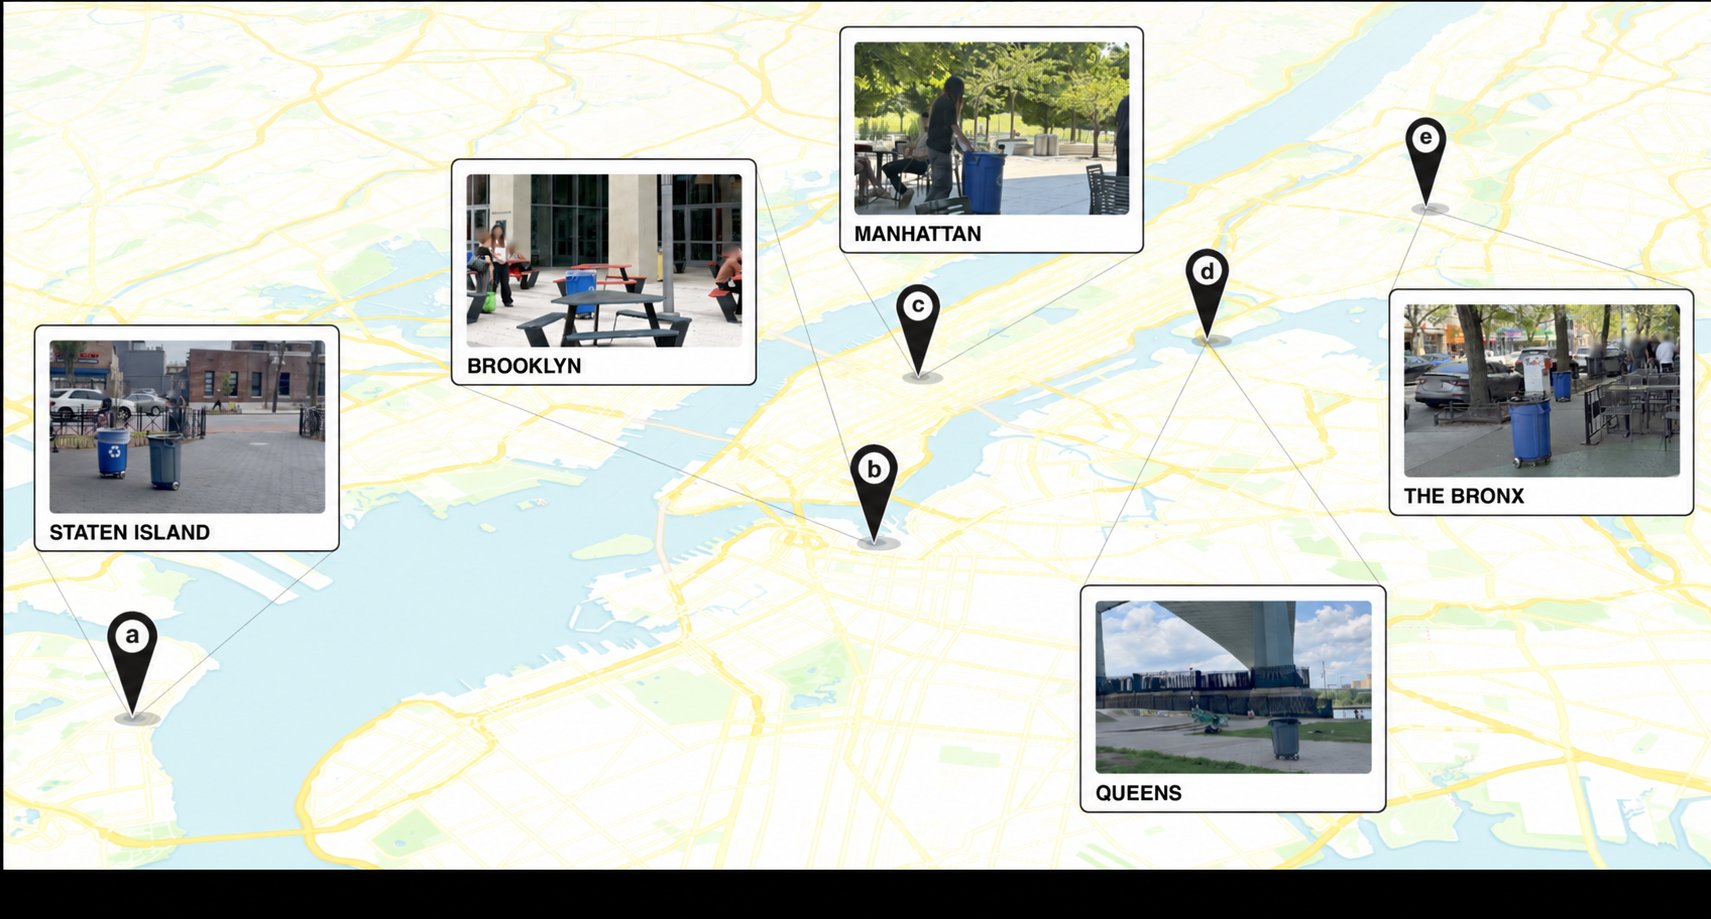
\includegraphics[width=\textwidth]{figures/teaser_mape.png}
  \caption{Trashbot deployments across New York City's five boroughs. The callouts show one deployment setting in each borough: (a)~Staten Island, (b)~Brooklyn, (c)~Manhattan, (d)~Queens, and (e)~the Bronx. Basemap \textcopyright{} OpenStreetMap contributors, \textcopyright{} CARTO.}
  \Description{A map of New York City with five photographic callouts, one for each borough. The callouts show TrashBots in a park in Staten Island, a seating area at the Brooklyn Navy Yard, an campus caf\'e seating area in Manhattan, a riverside park in Queens, and an outdoor commercial seating area in the Bronx.}
  \label{fig:teaser}
\end{teaserfigure}

\maketitle

% Basemap credit for Fig.~\ref{fig:teaser}: required by the OpenStreetMap
% ODbL and CARTO's basemap terms. Unnumbered footnote on the first page.


\section{Introduction}

Autonomous robotic systems are moving out of the laboratory and into shared public space~\cite{jung2018robots, pelikan2024encountering}. Delivery robots now roam city sidewalks~\cite{starship2025, yu2024understanding}, delivery drones ferry packages over residential neighborhoods~\cite{faa2025drone}, and driverless taxis carry passengers through downtown streets in cities around the world~\cite{waymo2025rides}. As these systems scale from isolated pilots toward routine presence, public frustration has also become visible. Residents have reported that delivery robots clutter street corners or block crosswalks~\cite{han2024codesign, yu2024understanding}, while some public encounters have involved obstruction or vandalism~\cite{sfstandard2024waymo, brscic2015escaping}. These encounters raise questions about how people read a robot's actions, work out what it is doing, and judge whether it belongs in a particular place.

Roboticists have long sought to deploy robots in public spaces, and HRI researchers have increasingly begun to examine how people might accommodate and make sense of these public robot encounters.~\cite{pelikan2024encountering,ekman2026sharing,bu2025making,weiss2010robots,jensen2005robots, thrun2000interaction} 
Pelikan et al. recently identified aspects of public sites and how they should inform robot design~\cite{pelikan2025localism}. However, it is often the case that a base robot platform is designed to be deployed in multiple locations. This work raises the question of whether the same robot remains equally legible across deployment sites. Comparing how people read the same service concept across settings can show which parts of an interpretation arise from the robot and which depend on the place in which it is encountered.

We pursue this question through a qualitative field study using two mobile Trashbots across five deployment sites spanning all five boroughs of New York City, building on prior field studies of mobile trash-receptacle robots~\cite{bu2024field}. We used a Wizard-of-Oz setup and conducted post-encounter interviews with people who engaged with the robots to examine how they read the robots' actions and made sense of their presence~\cite{bu2025making}. Our sites included a riverside park in Queens, a commercial corridor in the Bronx, a neighborhood park in Staten Island, a campus caf\'e in Manhattan, and an industrial and commercial campus in Brooklyn (Figure~\ref{fig:teaser}). Together, the sites varied in everyday use, sanitation arrangements, institutional context, and degree of public access. The Trashbots served as a common \emph{design probe}\cite{boehner201214} across these settings. The study took place across 22 field days, during which the Trashbots encountered approximately 490 people. We collected 86 post-encounter interview records involving 115 people, all of which were included in the comparative analysis (Table~\ref{tab:sites}).

Our study addresses three research questions:


\begin{itemize}

\item \textbf{RQ1:} How do people ``read'' public service robots across our different sites?

\item \textbf{RQ2:} What strategies do people use to make sense of the robots' presence in their space?

\item \textbf{RQ3:} What factors influence how people read the robots' actions? Are they specific to the encounter site?

\end{itemize}

Our qualitative analysis examined how participants interpreted the Trashbots, the strategies they used to make sense of the robots' presence, and what informed these interpretations. We also drew on available onboard-camera footage to  characterize how people interacted with the robots during encounters.


Our findings motivate the development of the concept of \emph{local legibility} as a design objective for public service robots. We use the term to describe whether people can read a robot's actions and understand its role in relation to the place where they encounter it. This includes understanding what service the robot provides, who is responsible for it, what its sensing practices mean, and how it relates to existing activities, infrastructure, and services at the site. 

This work makes these contributions: \begin{itemize}  

\item We provide field observations of public robot encounters and post-encounter interviews
    across five sites in New York City. 
    
    \item We characterize the interpretive process through which people
make sense of public robots, identifying the shared questions
that structure this process across deployment settings. 

\item We show the knowledge and resource people draw on to address these interpretive process, producing different judgments about the robots across deployment settings.

 \item We derive design implications for local legibility: making robots’ purpose, institutional responsibility, and recording practices understandable within their settings, and adapting behavior and siting to local activities and needs.  \end{itemize}
\section{Related Work}
%intro 
 \subsection{Robots in Public and Urban Space}
  Robots have been moving beyond experimental prototypes confined to the laboratory, and gaining greater exposure in public spaces. Jung and Hinds' call for in-the-wild work capable of supporting robust theory marked this turn~\cite{jung2018robots}, and the intervening years have supplied deployments at increasing scale: sidewalk delivery robots now operate commercially~\cite{starship2025}, robotaxis carry a quarter of a million paid rides each week~\cite{waymo2025rides}, and drone delivery is moving from needing waiver to getting routine certification~\cite{faa2025drone}. Studying robots in public therefore matters because deployment changes both the conditions under which robots operate and what counts as successful operation~\cite{jung2018robots}. Outside the laboratory, robots sometimes enter spaces that were not designed around them and encounter people who have not been recruited, trained, or assigned roles in relation to them~\cite{rosenthal2020forgotten}. A robot should navigate and perform its intended task, while people around it must recognize what it is doing~\cite{hetherington2021hey}, decide how to move or act around it~\cite{weinberg2023sharing}, determine whether to help, avoid, or to use it~\cite{weiss2010robots}, and judge whether its presence is appropriate~\cite{bu2025making}.
  
  Field studies have examined how people accommodate, assist, and resist robots in shared spaces. Pedestrians negotiate passage with delivery robots that do not negotiate back~\cite{pelikan2024encountering, yu2024understanding}, compete with them for constrained sidewalk space~\cite{weinberg2023sharing, gehrke2023observed}, and sometimes step in when robots stall~\cite{dobrosovestnova2022little}; for people with mobility disabilities, such encounters could create additional navigation and accessibility challenges~\cite{han2024codesign}. Longer-term deployments similarly show that robots are understood and used differently depending on the people, workflows, and organizations around them~\cite{mutlu2008robots, lee2012ripple, lee2010gracefully}. Other studies in the field also examine breakdowns in public interaction, including cases where people obstruct, damage, or otherwise resist robots: children obstruct and abuse social robots in malls~\cite{brscic2015escaping, nomura2016why}, passers-by push and strike robots in public squares~\cite{salvini2010safe}, and crowds have vandalized autonomous vehicles~\cite{sfstandard2024waymo}. 

  Beyond these direct forms of engagement, robots also affect people who are simply present in the surrounding environment. A related body of work examines such bystanders, who encounter robots without being recruited into interaction, distinguishing them from operators and supervisors~\cite{scholtz2003theory}. Privacy-focused works examine what robots record, who receives those data, and how such information is retained~\cite{rueben2018themes, lutz2019privacy, dietrich2026bystander}. Empirical work further shows that privacy judgments depend on how sensing is framed and on the norms of the setting~\cite{butler2015privacy, denning2014insitu}, consistent with contextual integrity's account of privacy as context-dependent information flow~\cite{nissenbaum2010privacy}.
  
  % Ours is the opposite arrangement: a robot that stays only hours, in six settings, so that what varies is the place rather than the length of the acquaintance.
  
  % A second strand documents what happens when the negotiation fails. Children obstruct and abuse social robots in malls, and asked why, give reasons that are about the robot's perceived agency and about the situation they are standing in~\cite{brscic2015escaping, nomura2016why}; a robot left to move through an Italian city square is pushed, blocked and struck by passers-by~\cite{salvini2010safe}; a Waymo vehicle is set alight by a crowd in San Francisco~\cite{sfstandard2024waymo}. Such incidents are typically narrated either as isolated pathology or as evidence of diffuse public hostility toward automation. Neither reading asks what the robot was taken to \emph{be} at the moment it was attacked, which is the question we think does the explanatory work.
  
  % A third strand concerns the people a public robot records without recruiting. Scholtz's early taxonomy of HRI roles already separates the bystander---present in the robot's space, with no task relationship to it and no way to opt out---from the operator and the supervisor~\cite{scholtz2003theory}, and the privacy literature has since made that position its central problem: what a robot sees, who receives it, and on what terms it may be retained~\cite{kaminski2017averting, rueben2018themes, lutz2019privacy, dietrich2026bystander}. Empirical work here tends to find that concern tracks the framing and the setting rather than the sensor: people asked about a teleoperated home robot's camera respond to how the capability is described~\cite{butler2015privacy}, and bystanders of wearable cameras in public reason about the norms of the specific place they are standing in rather than about recording as such~\cite{denning2014insitu}. Nissenbaum's contextual integrity gives that observation its general form---a flow of information is appropriate or not relative to the norms of the context it occurs in, not in the abstract~\cite{nissenbaum2010privacy}. 
  
Across these lines of work, the challenges of public robot deployment extend beyond technical performance to a broader question of how robots become understandable, acceptable, and workable within existing social environments. Local norms shape what a robot is understood to be and what it is permitted to do~\cite{while2021urban}. The social dimension is therefore not secondary to deployment success, but constitutive of it: even a technically capable robot may fail in practice if people cannot make sense of its purpose or role in the setting. 
Our work builds on this view by examining how place enters into the interpretation of a public robot at the scale of everyday encounters. By deploying the same Trashbot design across sites, we examined how people drew on local social conditions to read the robots' actions and make sense of their role in the setting.
  
  \subsection{Situated Action and Local Context} \label{sec:situated}
A robot's meaning depends on the norms of the place it enters, thus people's reactions to it are \textit{situated}: read off the place as much as off the robot itself. People make sense of a situation by looking at what happened, using cues from the environment and their own experience to build an explanation that seems reasonable~\cite{suchman1987plans, weick2005organizing}. Applied to an encounter with an unfamiliar robot, interpretation draws on what they already know about that place. A robot's onboard camera may be read differently on a university campus than on a commercial street. This is not because the sensor differs, but because the two sites hand the bystander different resources for resolving the same inference~\cite{denning2014insitu}. Site, on this account, is not a backdrop; it supplies the local knowledge the judgment is built from.

Prior work has examined what this local knowledge consists of and how it shapes robot encounters at a given site. Pelikan's argument for \textit{localism} in robot design is the closest statement of the underlying commitment: public space is not a uniform substrate into which robots are inserted, and designing for it requires attending to the specific social organization of specific places~\cite{pelikan2025localism}. Bu et al.'s study of trash barrel robots and Pelikan et al.'s account of street encounters both demonstrate this empirically at a single site, identifying the cultural knowledge, communal common ground, and everyday activity that one place makes available to interpreters~\cite{bu2025making, pelikan2024encountering}. Localism establishes that place shapes interpretation, but it does not yet say what a robot should do to be understood within a given place. 

A related design goal already exists in HRI: \emph{legibility}. Dragan and colleagues define legible motion as motion from which an observer can readily infer a robot's goal, distinguishing it from predictable motion, which matches what an observer expects once that goal is known~\cite{dragan2013legibility}. This idea has since informed work on human-aware and socially aware navigation~\cite{kruse2013human, singamaneni2024survey}. In this literature, legibility is primarily a property of robot behavior: the central question is, \emph{what is this robot about to do?}   

A situated view of interpretation raises a different question: \emph{does the same robot behavior remain equally legible across places?} If people interpret robots using knowledge of the setting around them, then legibility may depend not only on what the robot does, but also on where it does it. Yet little prior work has examined how the interpretation of the same robot changes across local settings. We extend the idea of legibility in two ways. First, we examine the same robot across different sites, allowing us to study how interpretation varies as the surrounding place changes. Second, we turn localism into a design implication. If people across sites ask similar questions---who runs this, is it watching me, does it belong here---then the design challenge is to help the robot answer those shared questions in ways that make sense locally. We call this \emph{local legibility}.

  \subsection{Sensemaking in and beyond HRI}
We use \textit{sensemaking}~\cite{weick2005organizing,pirolli2011introduction} to describe the interpretive work through which people make an unfamiliar situation intelligible and decide how to respond; a process has typically been studied by controlling what the robot does and then asking how people interpret it. This framing shaped three interlocking methodological choices in our study: why we used a Wizard-of-Oz robot, why we situated it through naturalistic observation in a real public space, and why we analyzed interview responses as data about sensemaking.

First, within HRI, Wizard-of-Oz methods have supported a controlled-experiment tradition: by having a hidden operator drive a robot that is perceived as autonomous, researchers can hold its behavior constant while manipulating some other feature of the interaction or the observer, as in studies of the legibility and predictability of robot motion~\cite{dragan2013legibility}, or of how people form mental models and expectations of autonomous systems~\cite{paepcke2010judging, riek2012wizard}. 

Second, we complement this controlled behavioral apparatus with naturalistic observation of bystanders in uncontrolled public space. Previous studies have shown that interpretation occurs even without explicit interaction, as people observe, test, avoid, or otherwise respond to robots encountered in situ~\cite{pelikan2024encountering, sabanovic2006robots}. Because such deployments cannot control what the robot does or when a bystander encounters it, they trade behavioral control for ecological validity. Our approach draws on both traditions: we used the same Trashbot design and Wizard-of-Oz operating arrangement across sites while observing encounters in natural public settings. This allowed us to compare how people read a common service concept across settings while keeping the robot platform and operating arrangement broadly consistent.
  
Third, we treated the post-interaction interviews not as elicited evaluations of the robot but as a further site of sensemaking in their own right. This follows Clark's claim that interpretation depends on what interlocutors take as shared ground~\cite{clark1996using}, and Madsbjerg's argument that people reason through data that is ``thick'' with context rather than abstracted from it~\cite{madsbjerg2017sensemaking}: an interview response is not a transparent readout of what someone thought while encountering the robot, but a further act of sense-making, produced after the fact and shaped by what the person now takes to be relevant. We therefore let the questions we asked stay open, and let the categories we analyzed emerge from what people actually said, rather than fixing in advance which aspects of the robot were worth asking about. The resulting data speak less to how people rated the robot than to what they reached for in order to explain it to themselves and to us--- prior experience with robots, guesses about who was operating it, assumptions about the sites, which is the kind of evidence a closed-ended survey would not have surfaced.
  
  % The term \emph{sensemaking} reaches HCI largely through Weick's account of % organizing, where it names the ongoing work by which people build plausible % accounts of situations that do not interpret % themselves~\cite{weick2005organizing}. HCI has its own lineage for the term--- % sensemaking as the cost-structured work of finding and encoding a representation % that fits a task~\cite{russell1993cost}, and as the gap-bridging people do when a % situation stops cohering~\cite{dervin1998sense}---but Weick's version is the one % that carries the features we need. Three of them bear % directly on what follows. Sensemaking is \emph{retrospective}: people act first % and work out what the action meant afterward, so the account and the conduct are % produced at different moments and need not agree. It is \emph{social}: accounts % are assembled for and with other people, and what settles them is plausibility % within a community rather than correspondence to some fact of the matter. And it % is \emph{ecological}: the materials people reason with are furnished by the % situation they are standing in, not retrieved whole from memory. Weick's % sensemaker is not a mind solving a puzzle but a person acting into an equivocal % world and talking about it as they go.
  % HRI has adopted the vocabulary while narrowing the construct. In much of the % field's usage, sensemaking names something a single person does internally during % an encounter: an inferential process running from cues on the robot's surface---its % form factor, its motion, its markings---to a conclusion about what the machine is % and what it wants. The unit of analysis is the individual; the timescale is the % encounter; the outcome is a mental model. This framing has been productive, and % the closest prior study of trash barrel robots in public space works within % it~\cite{bu2025making}, as does the broader literature on how bystanders read % robots they meet on the street~\cite{pelikan2024encountering}. But it quietly % drops two of Weick's three features. The social production of the account % disappears into individual cognition, and the environment shrinks to the robot % itself---a source of stimuli rather than a source of interpretive resources.
  % Our contribution is in part a recovery. We argue that the environment people % recruit when they make sense of a public robot is not the robot but the % \emph{place}: its history, its reputation, the work that maintains it, the bodies % that occupy it, the institutions understood to be operating in it. Restoring the % setting to the analysis changes what counts as an explanation of cross-community % difference. If sensemaking is an individual cognitive act, differences between % neighborhoods must be explained by differences between the people in them---by % attitudes, familiarity, or demographics that individuals carry with them. If it % is a situated practice, the same explanation is available without that % commitment: the practice is shared, and the difference lies in what each place % puts within reach. % \note{Verify the characterization of \cite{bu2025making} and % \cite{pelikan2024encountering} against the actual papers before submission --- % this paragraph asserts what framing they adopt, and a reviewer who knows either % work will check. If Pelikan et al.\ are already closer to a situated reading than % implied here, soften to cite them as a partial precedent rather than an instance % of the narrow framing.}
 
\section{Method}
\label{sec:method}

\subsection{Trashbots as a Probe}
\label{sec:probe}

We used two Trashbot as field probes to study how members of the public read and evaluate a mobile service robot encountered in everyday public space. The Trashbots provided a concrete service that participants could recognize and respond to~\cite{bu2023trash}, while their robotic capabilities invited further interpretation. Their trash-receptacle form suggested a familiar sanitation function, while mobility, onboard camera, and apparently autonomous movement raised questions about what the robot was doing, how it worked, and whether such a system was appropriate or useful in that setting.

This combination made the Trashbots useful for eliciting views about public service robots through actual encounters. Participants could watch a robot move, decide whether to approach or use it, notice its camera and other visible features, and then describe what they understood its actions and presence. The probes therefore grounded participants' accounts in encounter with a functioning service concept.

The two Trashbots followed the same design: a cylindrical trash receptacle mounted on a mobile base, with an onboard camera positioned above the rim (Figure~\ref{fig:Trashbot}). We used a Wizard-of-Oz arrangement throughout the deployments. A researcher controlled each Trashbot from out of view so that people encountered an apparently autonomous mobile service robot. We kept the platform design and operating arrangement consistent across deployment sites.

Using the same probe design across sites allowed us to examine how the setting entered participants' interpretations. The Trashbot's physical form and service concept remained consistent while the surrounding setting changed. We could therefore compare how people read the same service concept in relation to different local conditions.

\begin{figure}[tbp]
    \centering
    \begin{subfigure}[t]{0.54\linewidth}
        \centering
        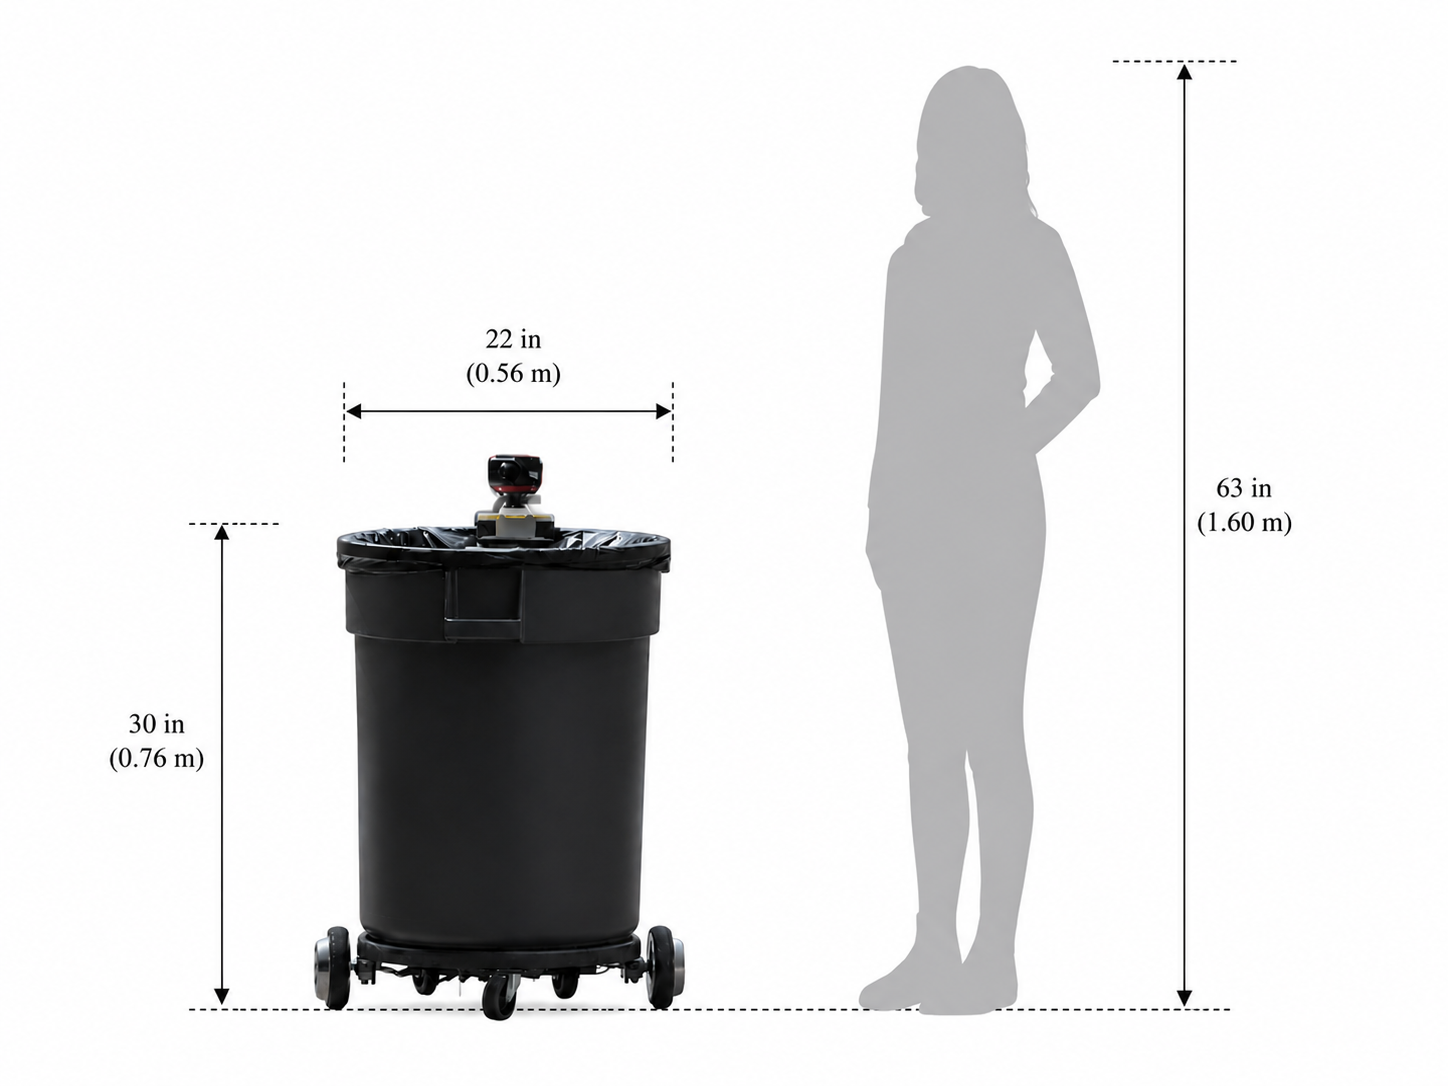
\includegraphics[width=\linewidth, trim=80 35 125 35, clip]{figures/Trashbot_compare.png}
        \caption{Trashbot at scale}
        \label{fig:Trashbot-scale}
    \end{subfigure}\hfill
    \begin{subfigure}[t]{0.43\linewidth}
        \centering
        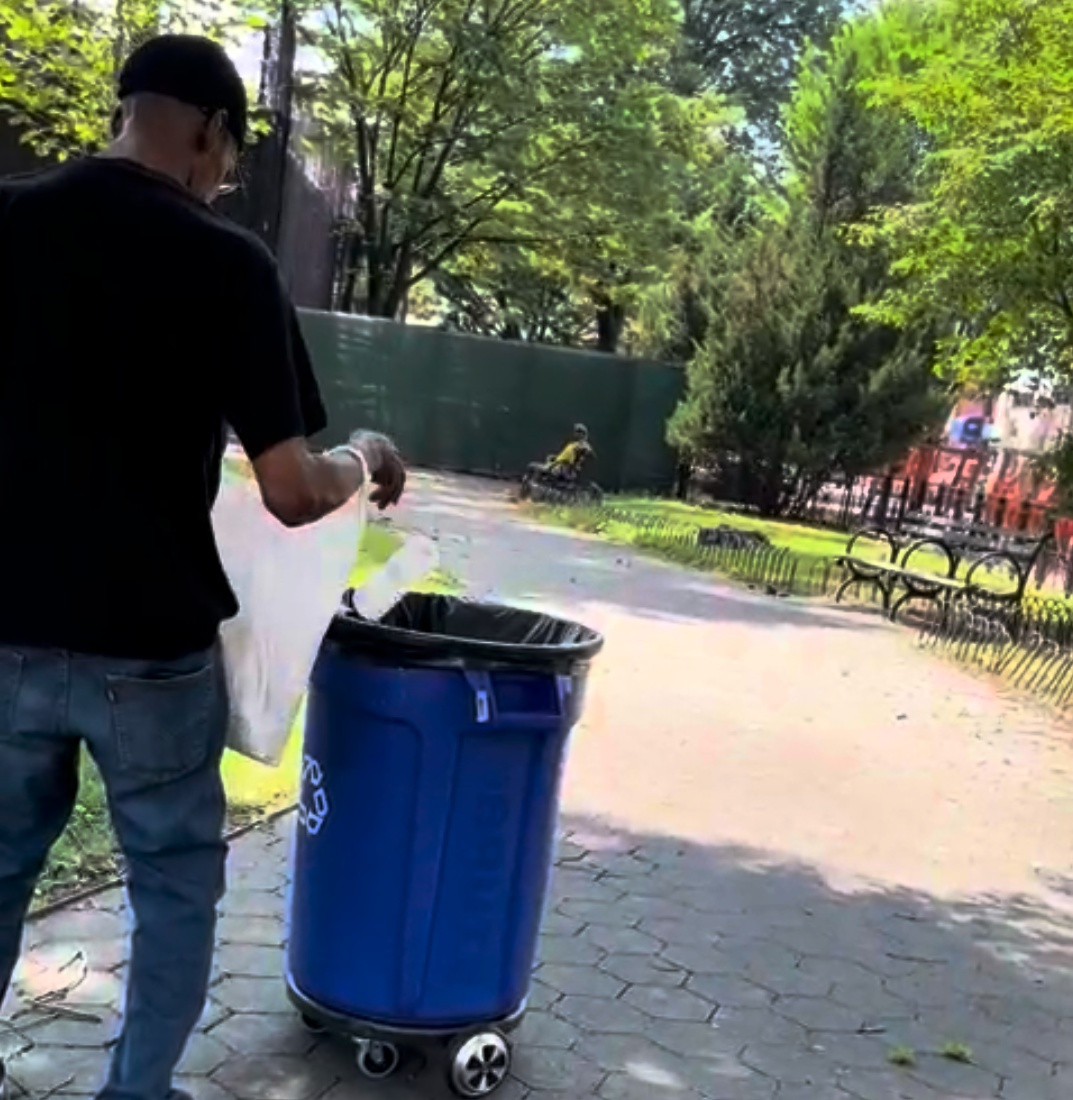
\includegraphics[width=\linewidth]{figures/example_encounter_TP-P03.jpg}
        \caption{Example encounter at Tappen Park}
        \label{fig:Trashbot-encounter}
    \end{subfigure}
    \caption{The Trashbot probe design. (a)~A Trashbot shown at scale next to a person. (b)~A participant at Tappen Park deposits a bag into a Trashbot during an encounter.}
    \Description{Two panels. The left panel shows a Trashbot next to a human silhouette for scale. The Trashbot is a cylindrical trash receptacle on a mobile base with a camera mounted above the rim. The right panel shows a participant at Tappen Park depositing a bag into a Trashbot during a field encounter.}
    \label{fig:Trashbot}
\end{figure}

Prior work has used mobile trash-receptacle robots to study encounters with service robots in public settings~\cite{bu2023trash,brown2024trash,bu2025making}. We use the same approach here to examine how public responses to a service robot vary across deployment sites.
  
\subsection{Deployment and Data Collection}
\label{sec:data-collection}

We deployed Trashbots at five sites across New York City's five boroughs: Tappen Park in Staten Island, Astoria Park in Queens, Little Italy in the Bronx, a cafe at a research institute in Manhattan, and the Brooklyn Navy Yard in Brooklyn. The sites included neighborhood and leisure parks, a commercial corridor, and institutional or commercial campus settings. We selected this set to place the same robot in public settings that differed in spatial organization, patterns of use, and existing service arrangements while remaining within one metropolitan context. Public-park deployments were conducted under a New York City Department of Parks and Recreation research permit. Access to the remaining sites was arranged with the organizations or people responsible for those spaces (see Appendix~\ref{app:sites}). Table~\ref{tab:sites} summarizes the deployment and interview corpus, and Figure~\ref{fig:sites} shows the five deployment locations.

Site selection was purposive rather than experimental. We chose settings that differed in everyday use, sanitation and maintenance arrangements, degree of public access, and institutional context. Feasibility also shaped the final set because each deployment required either a formal research permit or cooperation from the people responsible for the site. 

The sites are not matched conditions. Setting type, local population, degree of public access, sanitation infrastructure, and institutional context vary together across locations, so the study cannot isolate the effect of any one factor. We do not treat site as an independent variable or use these data to estimate neighborhood-level differences in acceptance or behavior. Instead, we use site as context for interpreting what participants believed the Trashbot was, who they thought was responsible for it, what risks they associated with it, and whether they thought it fit the surrounding environment.

The study was approved by our institution's IRB(protocol number omitted for anonymous review). Across the five sites, we conducted 22 field days between April 2025 and August 2026. During each deployment, a Trashbot moved through the accessible public area of the site, approached people, stopped nearby, and continued through the space. People were free to use the receptacle, approach the robot, move away from it, gesture or speak toward it, or ignore it. We did not recruit people before these encounters because doing so could have changed how they interpreted or interacted with the robot.

After an encounter, a researcher approached people and invited them to participate in a short semi-structured interview. Consent was also obtained at that point, after the participant had already encountered the Trashbot. Interviews generally lasted three to five minutes, with longer interviews continuing when participants had more to discuss. The interview guide asked about participants' first impressions, what they thought the Trashbot was doing, how they understood its operation, and their views on having a system like it in the surrounding setting. Follow-up questions asked participants to explain the basis for their judgments when relevant. Interviews were video recorded when consent permitted and otherwise recorded in audio only. We retained and analyzed onboard-camera footage only for participants who permitted recording during consent.

Across the field deployments, the Trashbots encountered approximately 490 people. Several interviews involved pairs or small groups, so interview records and the number of people interviewed are not equivalent. The study involved 115 interview participants in total. The analyzed corpus contained 86 interview records from the five sites. We use the interview record as the unit reported in the quantitative code summaries; one record can therefore contain the views of more than one person.

\begin{table*}[tbp]
\centering
\caption{Trashbot deployment sites and interview corpus.}
\label{tab:sites}
\small
\setlength{\tabcolsep}{3pt}
\renewcommand{\arraystretch}{1.18}
\begin{tabularx}{\linewidth}{@{}
  >{\raggedright\arraybackslash}p{0.11\linewidth}
  >{\raggedright\arraybackslash}p{0.17\linewidth}
  >{\raggedright\arraybackslash}X
  >{\raggedright\arraybackslash}p{0.13\linewidth}
  cc@{}}
  \toprule
  \textbf{Borough} & \textbf{Site} & \textbf{Setting} & \textbf{Dates} &
  \makecell[t]{\textbf{Field}\\\textbf{days}} &
  \makecell[t]{\textbf{Interview}\\\textbf{records}} \\
  \midrule
  Staten Island & Tappen Park & Neighborhood park & Jul 2025 & 4 & 10 \\
  \addlinespace[3pt]
  Queens & Astoria Park & Riverside leisure park & Jul 2025 & 4 & 13 \\
  \addlinespace[3pt]
  Bronx & Little Italy & Commercial corridor & Apr--Oct 2025 & 7 & 32 \\
  \addlinespace[3pt]
  Manhattan & Campus caf\'e & Institutional caf\'e & Jul 2026 & 3 & 16 \\
  \addlinespace[3pt]
  Brooklyn & Brooklyn Navy Yard & Industrial / commercial campus & Jul--Aug 2026 & 4 & 15 \\
  \midrule
  \multicolumn{4}{@{}l}{\textbf{Total}} & \textbf{22} &
  \makecell{\textbf{86}} \\
  \bottomrule
\end{tabularx}

\par\smallskip
\begin{minipage}{\linewidth}
  \footnotesize
  Field days include all deployment days, including days without interview recruitment. Some interview records include pairs or small groups, for 115 people in total. 
\end{minipage}
\end{table*}

Field days and interview recruitment did not always coincide. Some deployments focused on observing encounters or engaging with the surrounding community and produced no interview records. We retain those days in the deployment count because they were part of the field study, while the interview analyses in Sections~\ref{sec:encounters}--\ref{sec:site-sensemaking} use the 86-record analytic corpus.

\begin{figure*}[t]
    \centering
    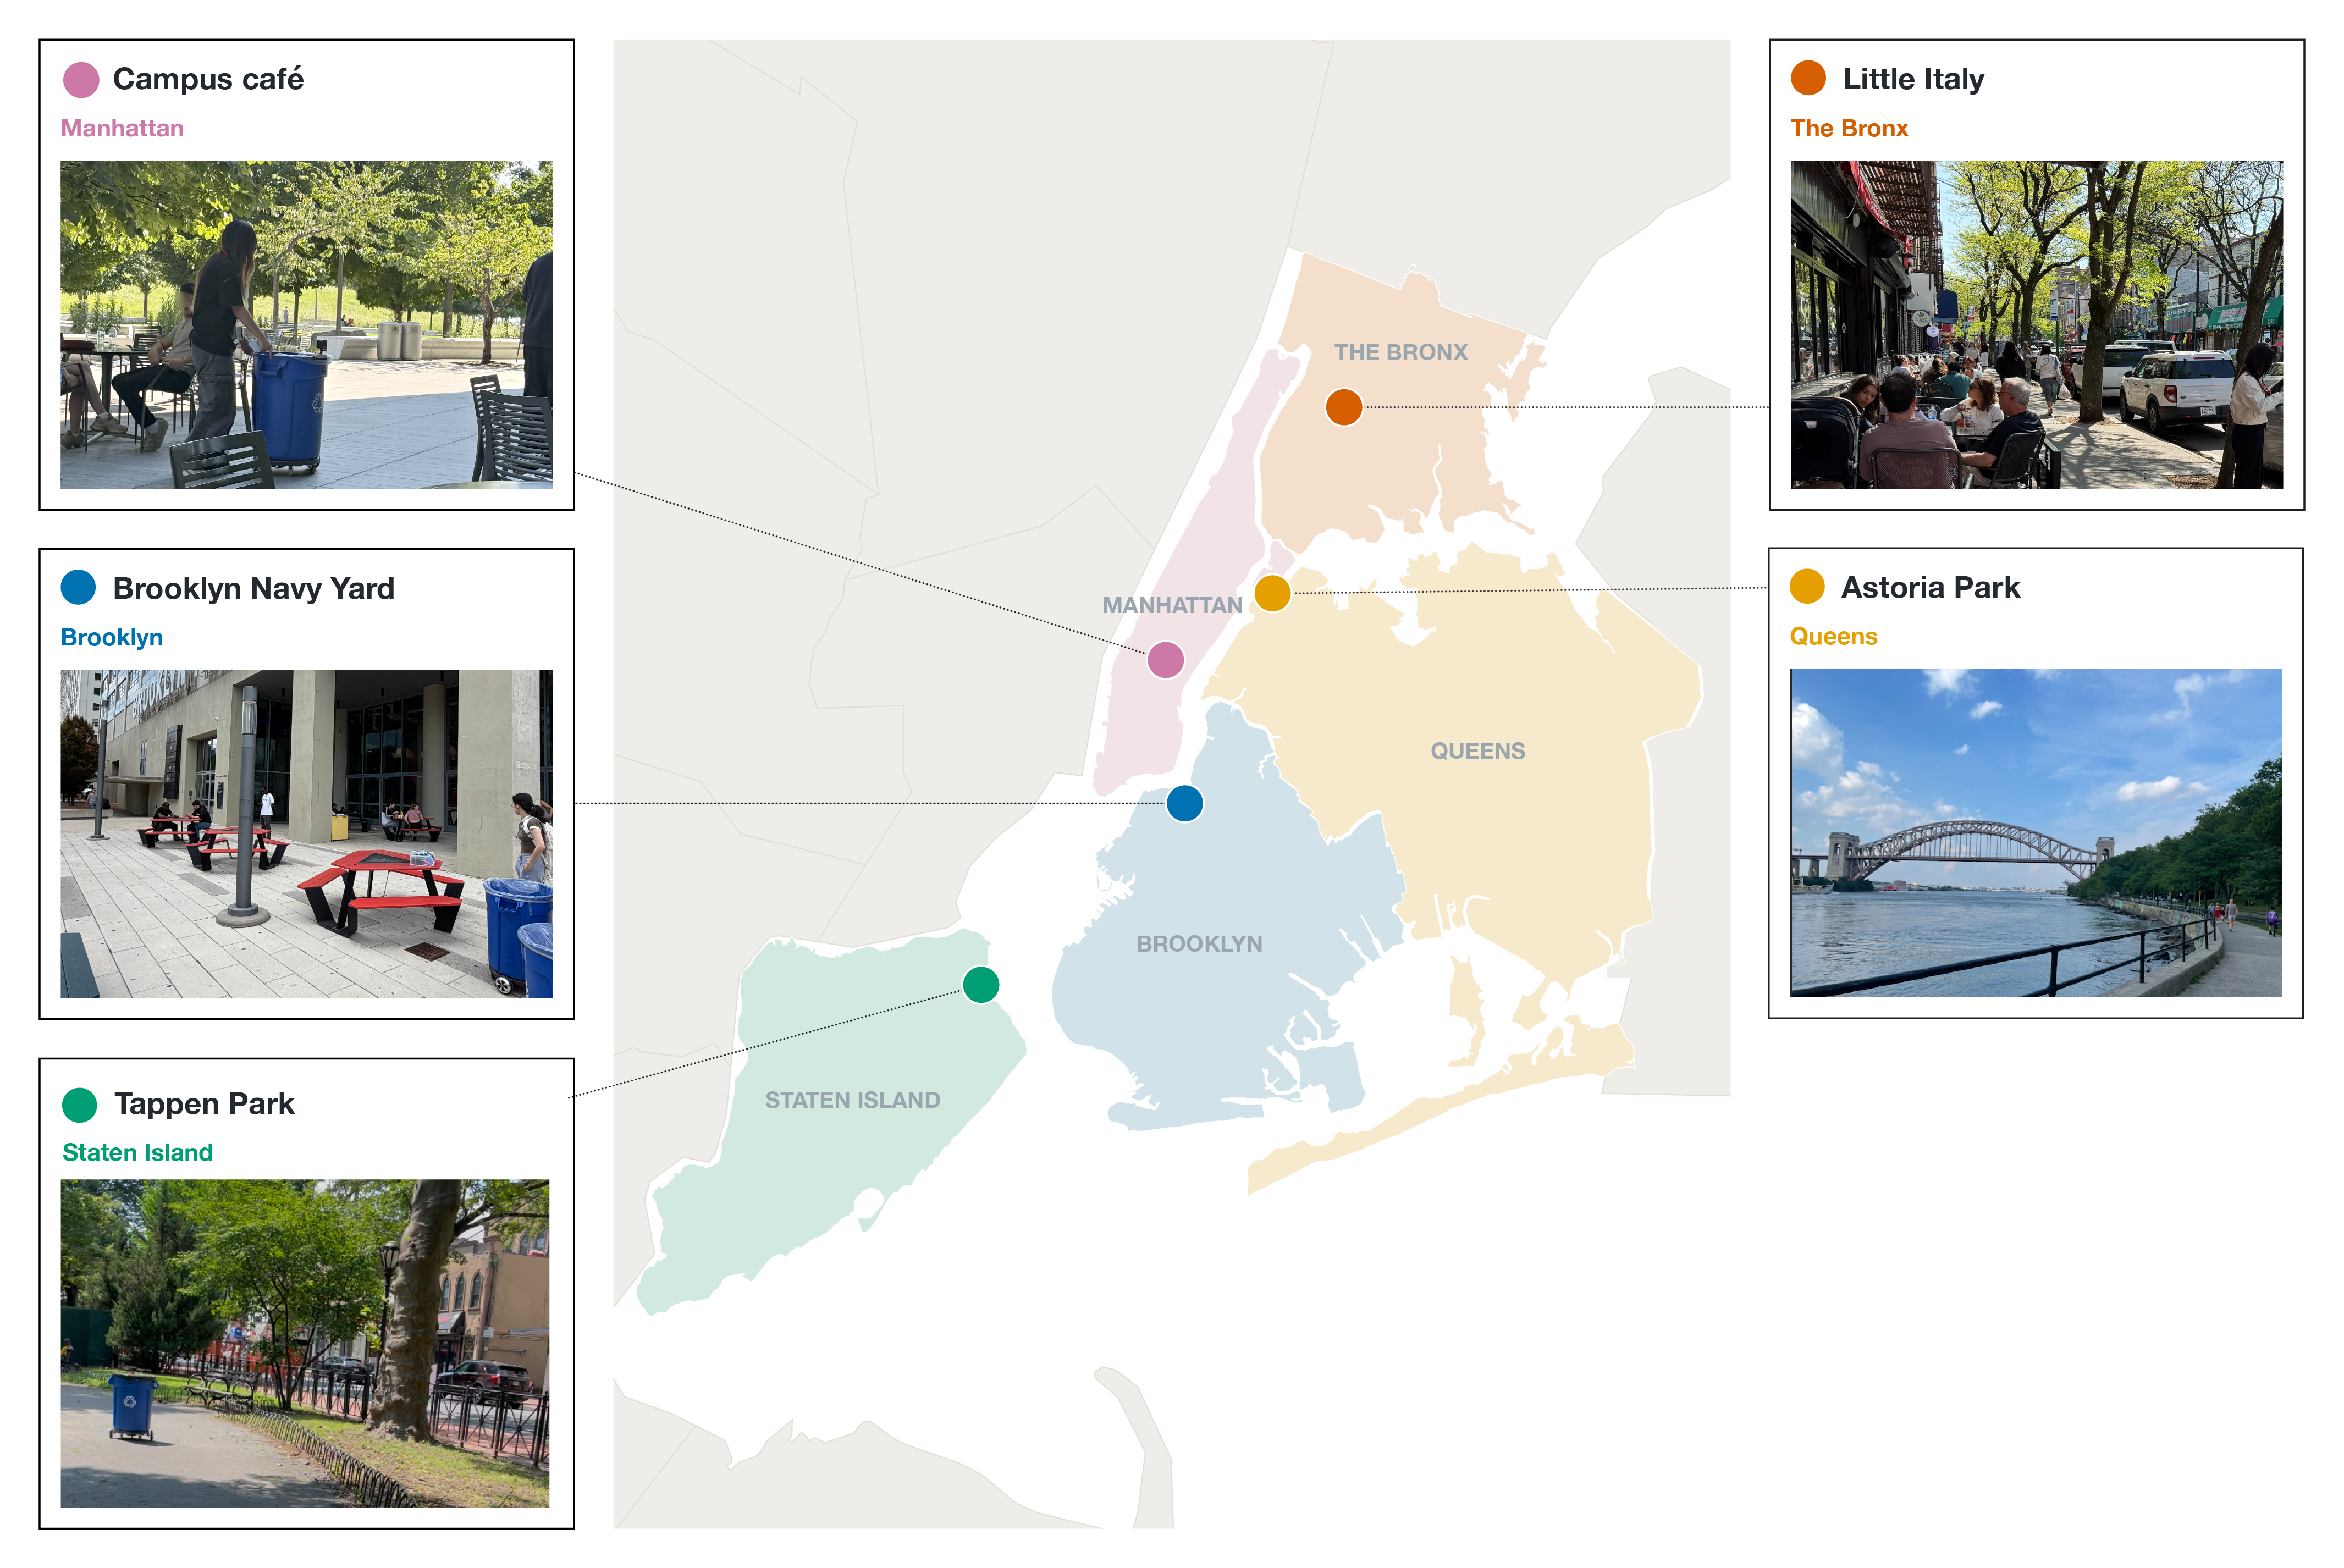
\includegraphics[width=\textwidth]{figures/sites_mapf.png}
    \caption{The five Trashbot deployment sites across New York City's five boroughs. The map shows Tappen Park in Staten Island, Astoria Park in Queens, Little Italy in the Bronx, the Campus caf\'e in Manhattan, and the Brooklyn Navy Yard in Brooklyn.}
    \Description{A map of New York City showing the five Trashbot deployment sites across five boroughs. Tappen Park is in Staten Island, Astoria Park is in Queens, Little Italy is in the Bronx, the campus cafe is in Manhattan, and the Brooklyn Navy Yard is in Brooklyn.}
    \label{fig:sites}
\end{figure*}

\subsection{Data Analysis}
Our analysis draws on records of participants' post-encounter interviews. The interview analysis identified the questions participants sought to resolve and the resources they drew on when interpreting the Trashbot. The interaction analysis characterized how encounters with the robot unfolded in practice. 
\subsubsection{Interview Analysis}
\label{analysis}
Three researchers independently reviewed the interview recordings and working transcripts, each developing a preliminary codebook. They then compared their proposed codes and collaboratively refined them into a shared codebook. The 86 interview records were distributed among the researchers using a round-robin procedure to balance site coverage across coders. Each researcher independently coded their assigned records using the shared codebook.

Following primary coding, we assessed intercoder agreement through independent double-coding of a subset of the interview records \cite{mcdonald2019reliability}. Each researcher coded an additional 15 records originally assigned to another researcher, with these secondary assignments distributed across sites. This procedure yielded 45 double-coded records, representing 52.3\% of the 86 interviews, with overlap covering all three coder pairings. Since the themes are not mutually exclusive, we
compute Cohen’s Kappa coefficient for each theme individually and average the coefficient across
themes. The resulting mean multi-label kappa coefficient is 0.72, which shows substantial agreement~\cite{ComputingInter-RaterReliability}.


\subsubsection{Interaction Analysis}
\label{sec:video-analysis}

Researchers manually reviewed each available onboard-camera recording. We treated the footage as interactional material rather than as a corpus of behavioral variables to be exhaustively coded and counted~\cite{jordan1995interaction}. Reviewers recorded these observations at the level of specific episodes and retained source files and timestamps where available. We used these observations to characterize how encounters unfolded and to identify moments that provided context for participants' later accounts.
\section{Findings}
\label{sec:findings}

We organize the findings around the three research questions. Section~\ref{sec:encounters} examines how participants read the Trashbots through their interactions and post-encounter accounts (\textbf{RQ1}). Section~\ref{sec:process} examines the strategies participants used to make sense of the robots' presence (\textbf{RQ2}). Section~\ref{sec:site-sensemaking} examines the factors that influenced how participants read the robots' actions and whether those factors were specific to the encounter site (\textbf{RQ3}). The comparative analysis includes 86 interview records from Tappen Park, Astoria Park, Little Italy, Campus Caf\'e, and Navy Yard. Participants are identified by site and interview number: TP for Tappen Park, AP for Astoria Park, LI for Little Italy, CC for Campus Caf\'e, and NY for Navy Yard.

\subsection{Encountering the Trashbot: Interactions, First Impressions, and Perceived Roles}
\label{sec:encounters}

To address \textbf{RQ1}, we examined how participants read the the Trashbots through observable interaction and through their post-encounter accounts of attitude, first impressions, and perceived roles. Figure~\ref{fig:rq1-pooled-codes} summarizes the prevalence of the interview codes across the 86 records, while Table~\ref{tab:codes-by-site-5-1} compares the same codes across deployment sites. Impression and perceived-role codes could co-occur within an interview record.

Encounters with the Trashbot were generally brief and opportunistic. People deposited waste when the robot came within reach, approached after watching how it moved, waved toward its camera, photographed or recorded it, or observed it from a distance. Figure~\ref{fig:site-encounters} shows examples from five deployment sites, one in each borough. At the campus caf\'e, CC-P04 recalled, \emph{``I didn't know what it was at first''}; nonetheless, he got up with an empty coffee cup and \emph{``slowly walked towards it.''} This account shows that interaction could begin while the robot's purpose was still uncertain.

\begin{figure*}[ht]
  \centering
  \begin{subfigure}[t]{0.30\textwidth}
    \centering
    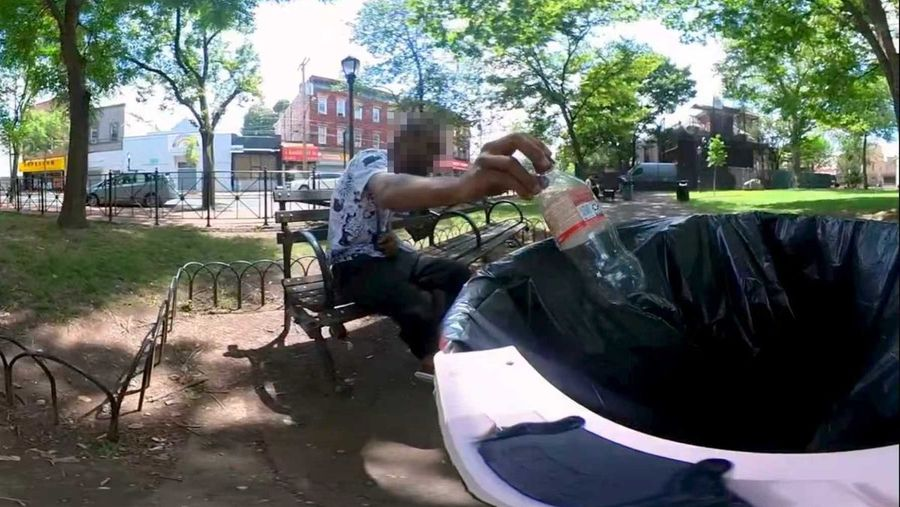
\includegraphics[width=\linewidth]{figures/vignettes/c_tappen_bottle.jpg}
    \caption{Tappen Park}
  \end{subfigure}\hfill
  \begin{subfigure}[t]{0.30\textwidth}
    \centering
    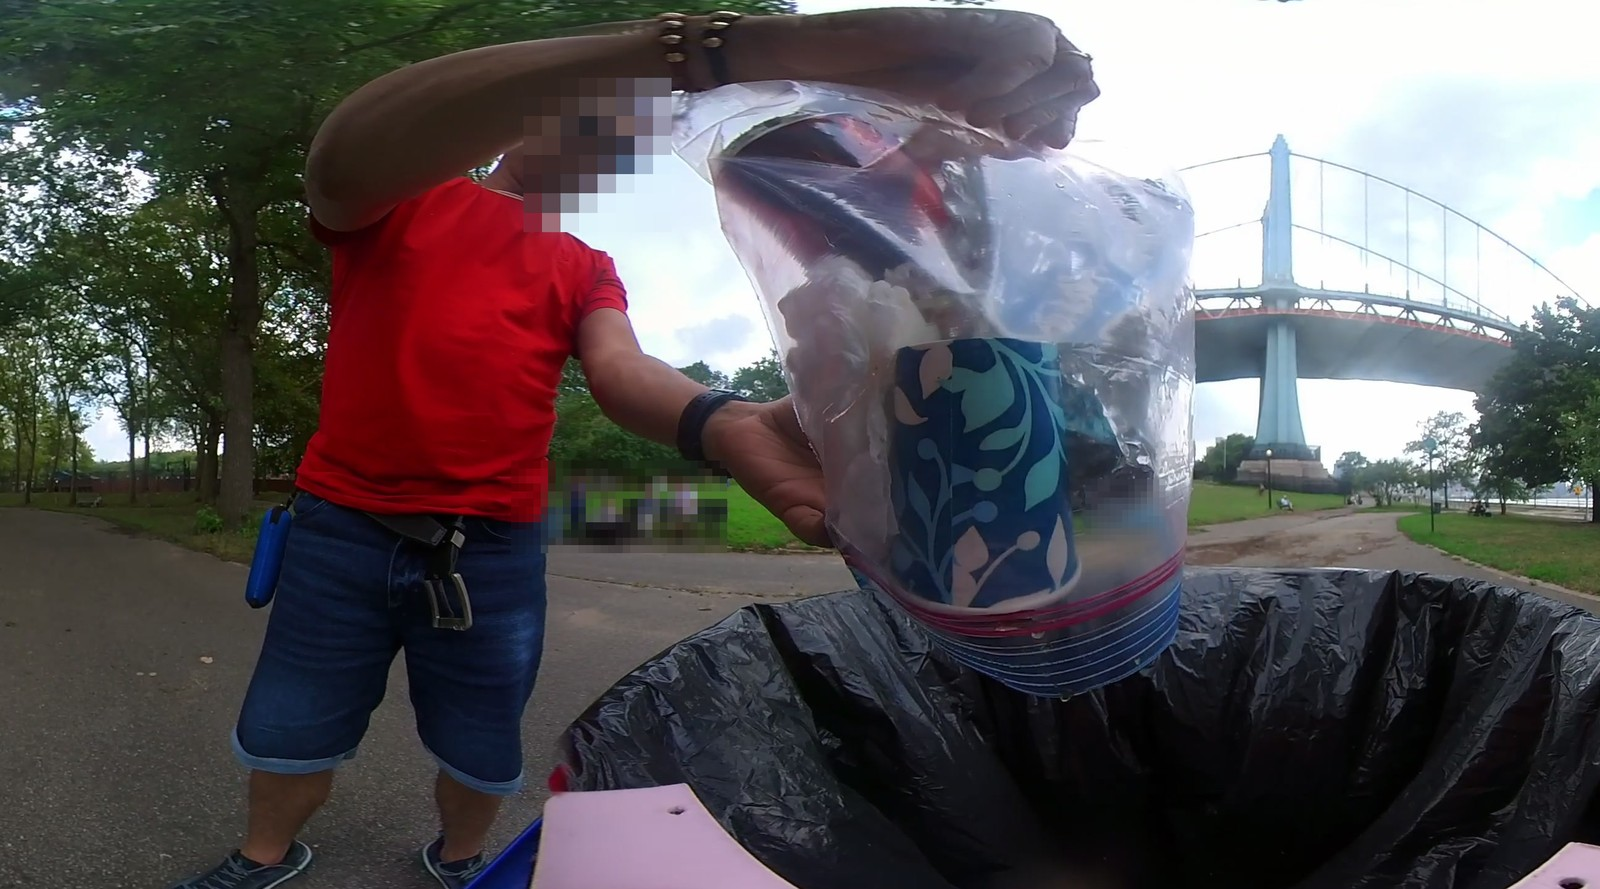
\includegraphics[width=\linewidth]{figures/vignettes/b_astoria_disposal.jpg}
    \caption{Astoria Park}
  \end{subfigure}\hfill
  \begin{subfigure}[t]{0.30\textwidth}
    \centering
    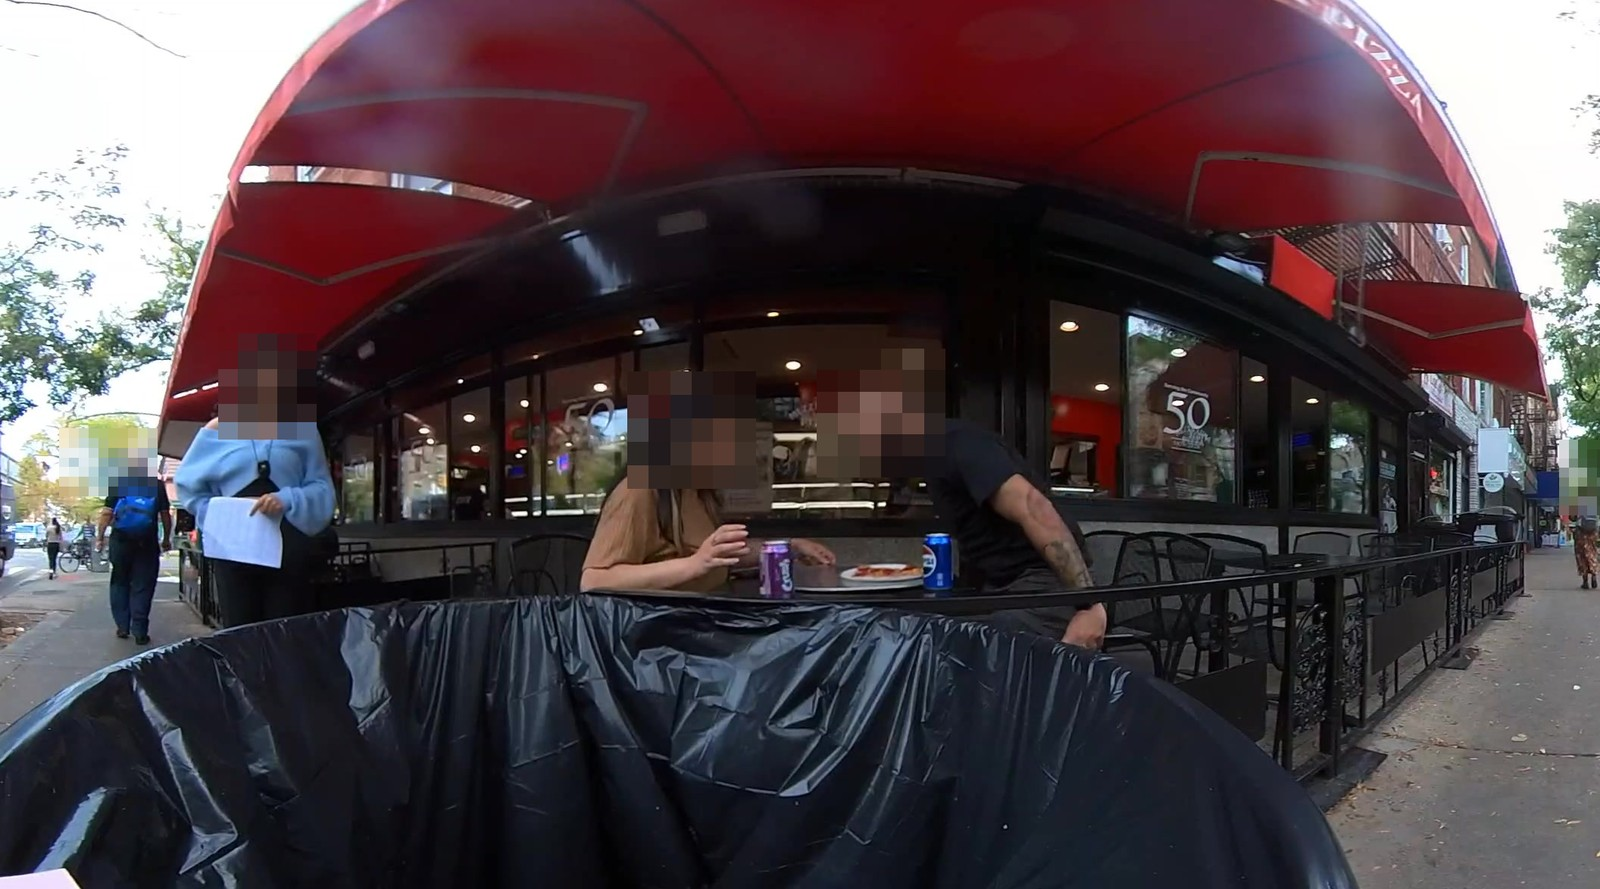
\includegraphics[width=\linewidth]{figures/vignettes/i_arthur_table.jpg}
    \caption{Little Italy}
  \end{subfigure}

  \medskip

  \begin{subfigure}[t]{0.30\textwidth}
    \centering
    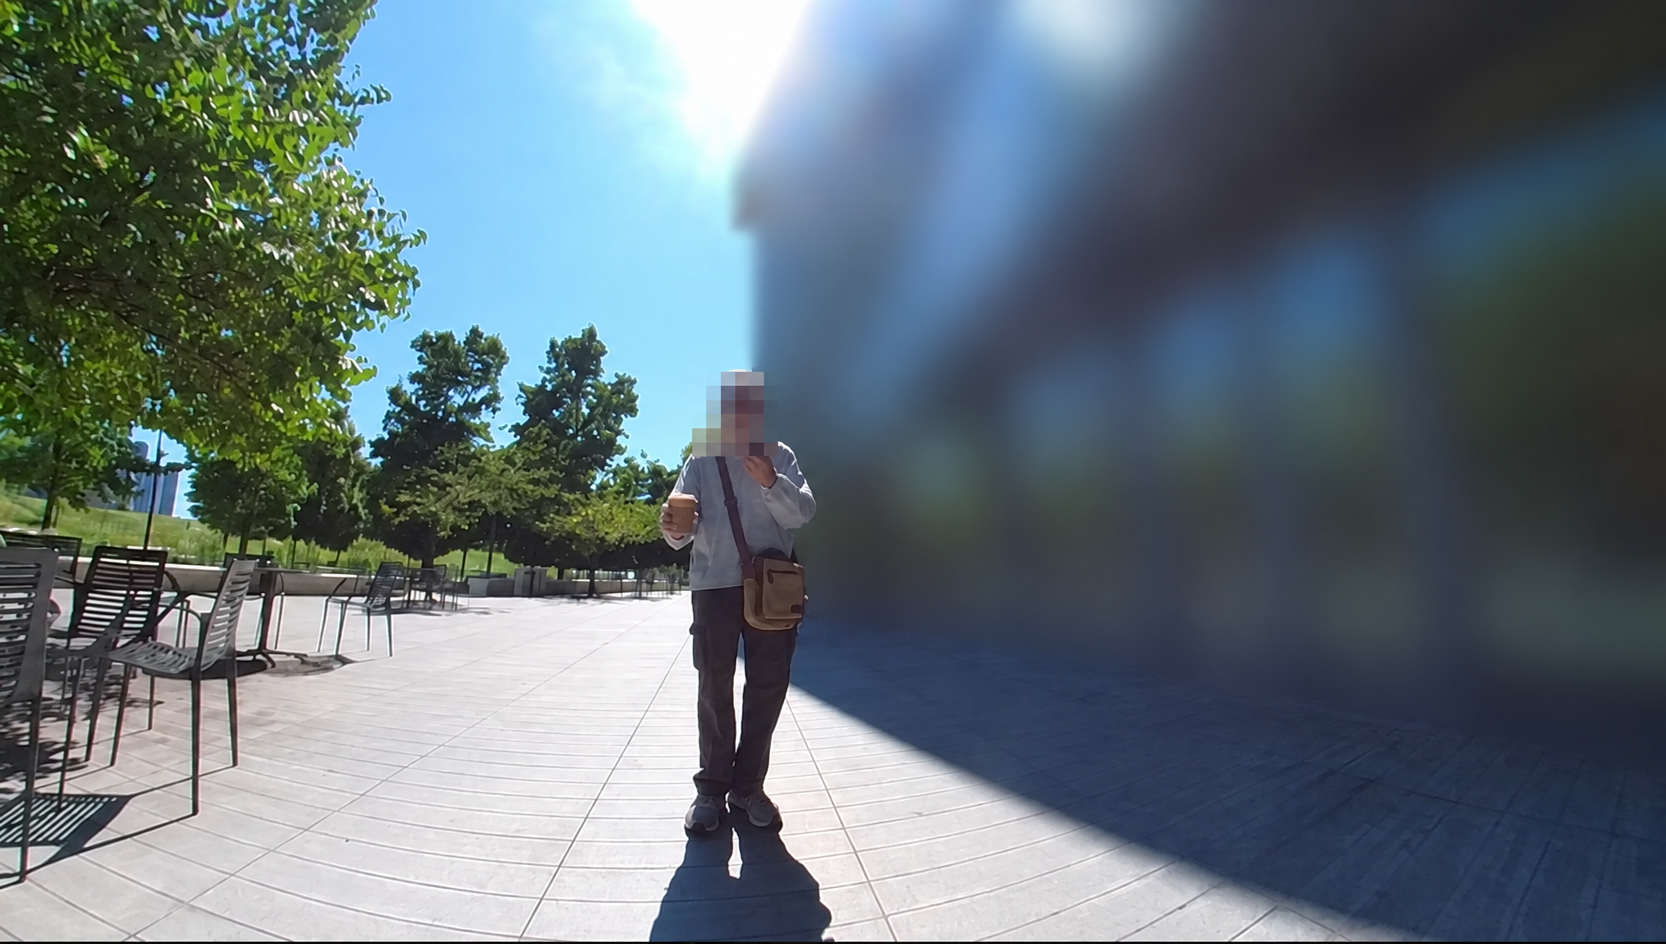
\includegraphics[width=\linewidth]{figures/vignettes/l_manhattan_cup.png}
    \caption{Campus caf\'e}
  \end{subfigure}\hspace{0.05\textwidth}
  \begin{subfigure}[t]{0.30\textwidth}
    \centering
    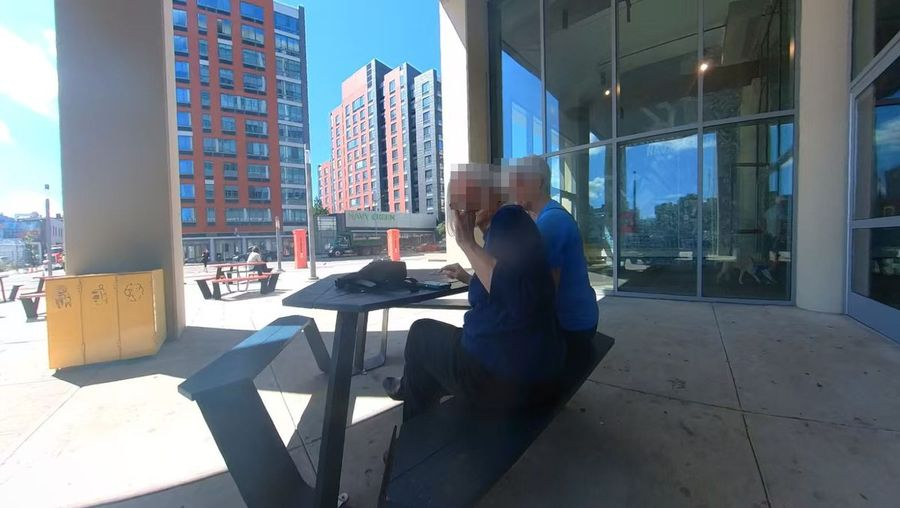
\includegraphics[width=\linewidth]{figures/vignettes/o_navyyard_wave.jpg}
    \caption{Brooklyn Navy Yard}
  \end{subfigure}

  \caption{Illustrative encounters with the Trashbot at five deployment sites, one in each New York City borough, viewed from the robot's onboard camera (faces obscured). At Tappen Park, TP-P07 reaches from a bench toward the receptacle with a bottle. At Astoria Park, AP-P02 empties a sealed bag into the receptacle. In Little Italy, the Trashbot stops beside a sidewalk table as LI-P26 reaches across its rim. At Campus Caf\'e, CC-P04 approaches while holding a coffee cup and a phone. At Navy Yard, NY-P08 gestures toward the onboard camera.}
  \Description{Five photographs from the Trashbot's onboard camera, showing encounters at one deployment site in each New York City borough. At Tappen Park, a person seated on a bench reaches toward the receptacle with a bottle. At Astoria Park, a person empties a bag into the receptacle on a park path. In Little Italy, a person seated at a sidewalk table reaches across the rim. At Campus Caf\'e, a person approaches while holding a coffee cup and a phone. At Navy Yard, a seated person gestures toward the camera. Faces are obscured.}
  \label{fig:site-encounters}
\end{figure*}

\begin{figure*}[ht]
    \centering
    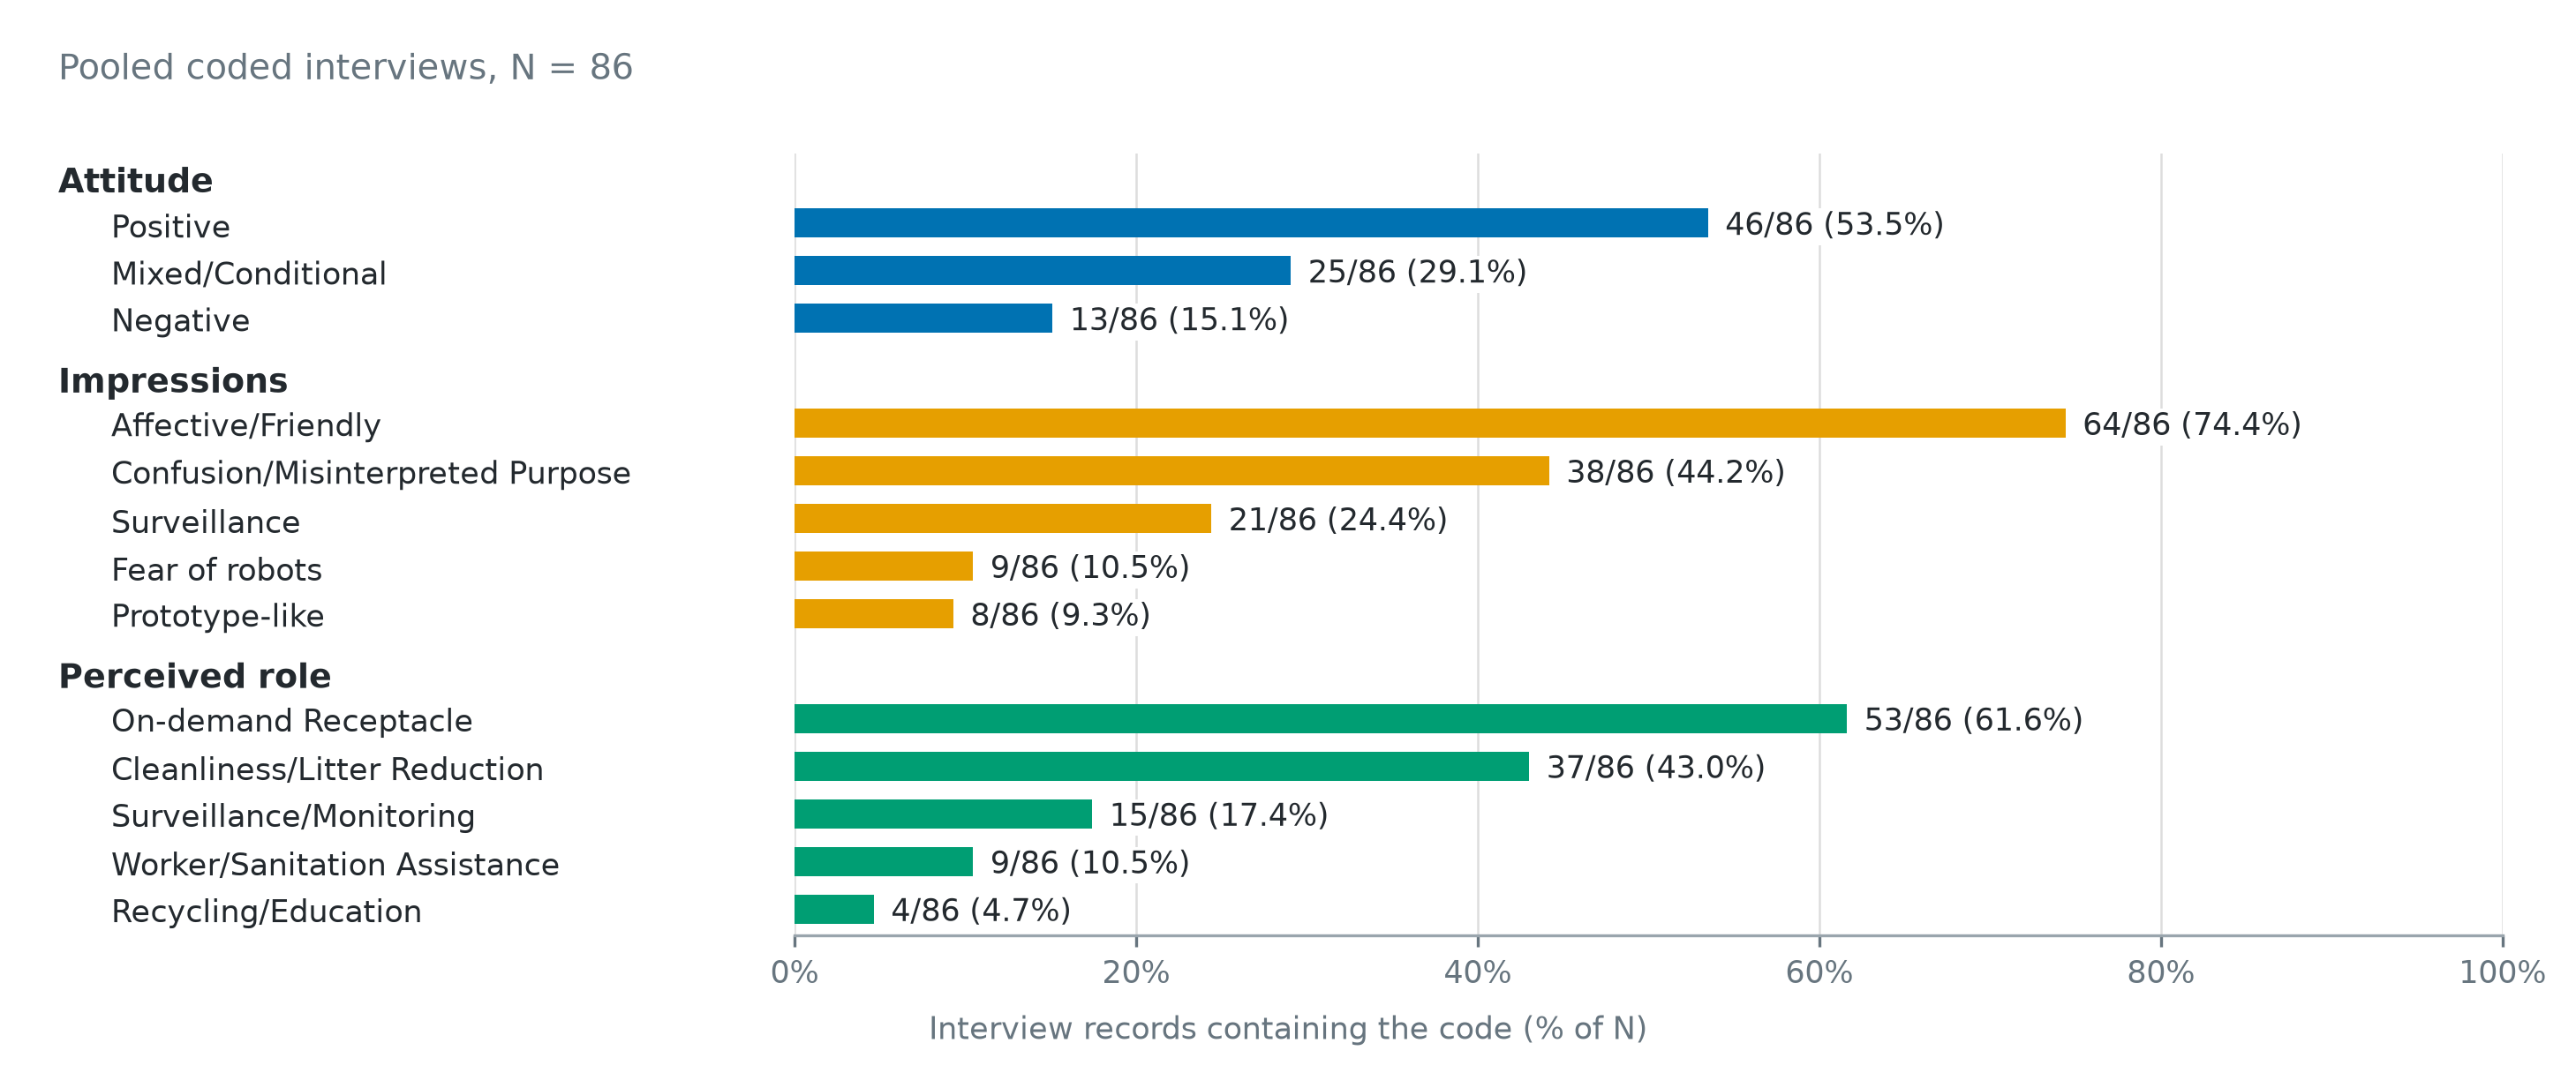
\includegraphics[width=0.95\textwidth]{figures/fig_5_1_all_sites.png}
    \caption{Prevalence of attitude, impression, and perceived-role codes across the pooled interview corpus ($N=86$ interview records). Bars show the share of records containing each code, so percentages within a group do not sum to 100\%.}
    \Description{Horizontal bar chart summarizing RQ1 interview codes across 86 records. Attitudes include 46 positive, 25 mixed or conditional, and 13 negative records. Impression codes include affective or friendly impressions in 64 records, confusion or misinterpreted purpose in 38, surveillance in 21, fear of robots in 9, and prototype-like impressions in 8. Perceived roles include on-demand trash receptacle in 53 records, cleanliness or litter reduction in 37, surveillance or monitoring in 15, worker or sanitation assistance in 9, and recycling or education in 4. Impression and perceived-role codes are nonexclusive.}
    \label{fig:rq1-pooled-codes}
\end{figure*}

\subsubsection{Attitudes}

Positive attitudes were the most frequent evaluation of the Trashbot. Forty-six of the 86 records (53.5\%) contained a positive attitude, 25 (29.1\%) contained a mixed or conditional attitude, and 13 (15.1\%) contained a negative attitude. Positive accounts commonly described the robot as useful, appealing, or appropriate for waste disposal. At the Brooklyn Navy Yard, NY-P10 called the Trashbot \emph{pretty cute} and later said, \emph{``I do like this one. I genuinely do.''}

Mixed or conditional attitudes combined approval with a condition on where or how the robot should operate. Participants raised issues such as pedestrian traffic, reliability, privacy, and the possibility of damage. AP-P04 expressed this distinction directly: \emph{``So, again, conceptually, I think it's a great idea. Practically, I think you're going to figure out where it works and where it doesn't.''} These participants often supported the service concept while reserving judgment about particular deployments.

Negative evaluations were less frequent. They included accounts that considered the robot unnecessary, unsuitable for a particular setting, or undesirable as a public technology. Attitude therefore captured participants' overall evaluation of the Trashbot, while more specific concerns about cameras, operation, or local fit were coded separately when present.

\subsubsection{Impressions}

Participants' first impressions of the Trashbot ranged from amusement and curiosity to uncertainty and concern. Affective or friendly impressions appeared in 64 of the 86 records (74.4\%), making this the most frequent impression code. Participants often described the robot as \textit{cool}, \textit{cute}, \textit{interesting}, or \textit{funny}, and some emphasized surprise at seeing a familiar object move through public space. AP-P01 recalled, \emph{``I was very curious.''} Fear of robots was much less common, appearing in 9 records (10.5\%). These reactions sometimes drew on broader concerns about autonomous systems, but they did not necessarily imply rejection of the Trashbot itself. A participant could find the encounter novel or appealing while still expressing unease about robots.

Confusion or a misinterpreted purpose appeared in 38 records (44.2\%). Participants could often identify the Trashbot as some kind of trash-related object while remaining unsure what its mobility, camera, or autonomy were meant to accomplish. In some cases, this produced an alternative interpretation altogether. AP-P13, for example, recalled, \emph{I was confused, I didn't know what it was for,''} adding that \emph{``it was like a toy.''} NY-P13 similarly suggested that \emph{``the trash can would need to be labeled.''} Prototype-like impressions, which appeared in 8 records (9.3\%), reflected a related uncertainty about the robot's status rather than its purpose: participants sometimes treated the Trashbot as an experimental object rather than a ready-to-use public service. AP-P04, for instance, assumed that \emph{``it's not the final product''} and asked whether \emph{``there's going to be more things ... added to this,''} later imagining what a more \emph{``manufactured version''} might look like. The camera introduced another interpretive possibility. Surveillance-related impressions appeared in 21 records (24.4\%), with some participants reading the robot not only as a service device but also as something that might record or monitor people. AP-P08 said that the robot \emph{``reminds me [of] robotic police,''} later connecting this impression to the camera and privacy concerns, while NY-P08 described the Trashbot as \emph{``a little startling.''} These reactions show that the robot's visible form provided an initial reference point without fully explaining either what its robotic features were for, whether it represented a finished public service, or what role its sensing might play.

\subsubsection{Perceived roles}

Participants most often understood the Trashbot in terms of what it could do for waste disposal and cleanliness, and these interpretations shaped whether the robot seemed useful. The most common role was an on-demand receptacle, appearing in 53 of 86 records (61.6\%). Here, participants understood mobility as making a trash can more accessible by bringing it closer to people. At the Brooklyn Navy Yard, NY-P11 asked whether the Trashbot was \emph{``going around so people can throw stuff in the garbage?''} and later said, \emph{``I could see it being useful.''} Cleanliness or litter reduction appeared in 37 records (43.0\%). LI-P03, for instance, said, \emph{``just to see any type of effort to clean up the streets is great, because we need that,''} noting that existing cans could be \emph{``overflowing or not available...or not maintained correctly.''} These two perceived roles often reinforced one another, since bringing a receptacle closer to users was one way participants imagined the robot contributing to cleaner public space.

Other roles focused on what the Trashbot's additional robotic features might enable beyond disposal itself. Surveillance or monitoring appeared in 15 records (17.4\%), extending the surveillance-related impressions described above. Whereas the visible camera could initially make the robot seem startling, some participants also saw it as serving a monitoring function. LI-P03, for example, described cameras as potentially useful for safety because \emph{``maybe people think twice before they come in a crime...''} The camera could therefore make the robot seem useful in an additional way. 

Worker or sanitation assistance appeared in 9 records (10.5\%). LI-P17, who identified themselves as a sanitation worker, explained, \emph{``It looks like it makes people's job [and] my job easier.''} They also weighed whether the robot might reshape sanitation work—allowing workers to focus on more demanding tasks while also raising the possibility that employers could reduce staffing. In this sense, the robot’s usefulness was judged in relation to existing labor arrangements. As we will present in Section~\ref{sec:site-sensemaking}, these judgments were also shaped by the services, staffing, and waste-management arrangements already present at particular sites. Recycling or educational roles were less frequent, appearing in 4 records (4.7\%). LI-P28 suggested that \emph{it would be really interesting to have one recycling can''} that could tell users, \emph{no, no, sorry, don't put that paper in here.''} In this account, the robot's usefulness extended beyond making disposal more accessible to helping guide how waste should be sorted. Overall, whether participants saw the Trashbot as an on-demand receptacle, a tool for reducing litter, a monitoring device, an assistant to sanitation workers, or a recycling aid, these perceived roles gave them different grounds for judging what the robot was useful for and what it added to the space during the encounter.

\subsubsection{Across sites}

Table~\ref{tab:codes-by-site-5-1} compares the RQ1 codes across the five deployment sites. Because impression and perceived-role codes could co-occur within an interview record, the table describes the prevalence of each interpretation rather than mutually exclusive groups.

\begin{table*}[t]
  \caption{Interview-code prevalence by site for RQ1. Each cell reports the number of interview records containing the code over the number of records represented at that site ($n/N$). Records may contain multiple codes or no applicable code within a category, so counts within each category need not sum to $N$. Sites: Tappen Park (TP), Astoria Park (AP), Little Italy (LI), Campus caf\'e (CC), and Brooklyn Navy Yard (NY).}
  \label{tab:codes-by-site-5-1}
  \small
  \begin{tabular}{@{}lcccccc@{}}
    \toprule
     & TP & AP & LI & CC & NY & All sites \\
     & $N=10$ & $N=13$ & $N=32$ & $N=16$ & $N=15$ & $N=86$ \\
    \midrule
    \multicolumn{7}{@{}l}{\textbf{Attitude}} \\
    \quad Positive & 7/10 & 8/13 & 14/32 & 10/16 & 7/15 & 46/86 \\
    \quad Negative & 0/10 & 1/13 & 7/32 & 2/16 & 3/15 & 13/86 \\
    \quad Mixed/Conditional & 3/10 & 3/13 & 11/32 & 4/16 & 4/15 & 25/86 \\
    \addlinespace
    \multicolumn{7}{@{}l}{\textbf{Impressions}} \\
    \quad Affective/Friendly & 7/10 & 9/13 & 27/32 & 13/16 & 8/15 & 64/86 \\
    \quad Confusion/Misinterpreted Purpose & 4/10 & 6/13 & 17/32 & 4/16 & 7/15 & 38/86 \\
    \quad Surveillance & 1/10 & 3/13 & 8/32 & 5/16 & 4/15 & 21/86 \\
    \quad Prototype-like & 0/10 & 3/13 & 2/32 & 3/16 & 0/15 & 8/86 \\
    \quad Fear of robots & 1/10 & 1/13 & 4/32 & 1/16 & 2/15 & 9/86 \\
    \addlinespace
    \multicolumn{7}{@{}l}{\textbf{Perceived role}} \\
    \quad On-demand Trash Receptacle & 5/10 & 8/13 & 18/32 & 11/16 & 11/15 & 53/86 \\
    \quad Cleanliness/Litter Reduction & 5/10 & 7/13 & 16/32 & 5/16 & 4/15 & 37/86 \\
    \quad Worker/Sanitation Assistance & 1/10 & 2/13 & 4/32 & 1/16 & 1/15 & 9/86 \\
    \quad Surveillance/Monitoring & 2/10 & 3/13 & 3/32 & 4/16 & 3/15 & 15/86 \\
    \quad Recycling/Education & 0/10 & 1/13 & 1/32 & 2/16 & 0/15 & 4/86 \\
    \bottomrule
  \end{tabular}
\end{table*}

Several patterns were shared across sites. Positive was the largest attitude category at each site, although its prevalence varied from 14 of 32 records in Little Italy to 7 of 10 at Tappen Park. Affective or friendly impressions were also the most frequent impression code at every site. The on-demand receptacle role appeared in half or more of the records at each site, with the highest proportions at the Brooklyn Navy Yard (11/15) and campus caf\'e (11/16). At Tappen Park, on-demand receptacle and cleanliness/litter reduction appeared equally often (5/10 each). These distributions indicate that participants across sites commonly recognized the Trashbot as an approachable waste-related service.

The distributions also differed in what participants found uncertain or salient. Confusion or a misinterpreted purpose appeared in 17 of 32 Little Italy records and 7 of 15 Brooklyn Navy Yard records, compared with 4 of 16 at the campus caf\'e. Surveillance impressions appeared at all five sites but were least frequent at Tappen Park (1/10). Prototype-like impressions were recorded at Astoria Park, Little Italy, and the campus caf\'e, but not at Tappen Park or the Brooklyn Navy Yard. Fear of robots remained uncommon across the corpus.

Perceived roles varied in a similar way. Cleanliness and litter reduction were especially prominent at Astoria Park (7/13), Little Italy (16/32), and Tappen Park (5/10), while fewer Brooklyn Navy Yard records assigned the Trashbot that role (4/15). Surveillance or monitoring appeared in 4 of 16 campus caf\'e records and in 3 of 15 Brooklyn Navy Yard records, compared with 3 of 32 in Little Italy. Worker assistance appeared at every site but remained uncommon, and recycling or education appeared only at Astoria Park, Little Italy, and the campus caf\'e.

The site-level comparison therefore shows a common starting point alongside different emphases. Across sites, participants often recognized a mobile waste-disposal service and responded to it positively or affectively. Their accounts differed more in what they thought the robot added to that familiar function. Some emphasized easier access to a receptacle or cleaner public space, while others attended to the camera, existing sanitation work, or uncertainty about why the trash can needed robotic capabilities. Section~\ref{sec:process} examines how participants developed these interpretations through questioning and reasoning.

\subsection{Interpreting the Trashbot: Question-driven and Reasoning-based Sensemaking} 
\label{sec:process}

We examined the interpretive strategies participants used to make the Trashbot’s presence intelligible in addressing \textbf{RQ2}. Among the strategies identified in our analysis, we focus here two broad forms that recurred across the data: \textit{question-driven sensemaking} and \textit{reasoning-based sensemaking}. Question-driven accounts surfaced uncertainty through WHAT, HOW, and WHO questions about the robot’s purpose, operation, and the actors behind it. Reasoning-based accounts instead worked through ambiguity by drawing inferences, projecting possible actions and consequences, and making analogies from available cues. Figure~\ref{fig:sensemaking-all-sites}a visualizes the percentage of interview records containing each interpretive-strategy code reported here.

\subsubsection{WHAT: identifying the robot and its role}
WHAT questions were raised by 33 participants (38.4\%), making them the most common question type. For some, these questions surfaced immediately; NY-P13 described \emph{``what does it do?''} as \emph{the first question.} These questions concerned identifying the Trashbot's function and role in the space. Typical WHAT questions included:

\begin{itemize}
    \item \emph{``What is this/What does it do?''} (\textit{e.g.}, AP-P04, LI-P22, NY-P10)
    \item \emph{``What is the point or purpose of it?''} (\textit{e.g.}, AP-P06, LI-P18, LI-P21)
    \item \emph{``What is the camera or collected data for?''} (\textit{e.g.}, LI-P01, TP-P04, NY-P15)
\end{itemize}

Some participants phrased similar uncertainties as WHY questions, such as \emph{``why a trash can needed to move?''}. We grouped these with WHAT questions because they likewise concerned the purpose of its robotic features. Participants were often able to recognize the Trashbot as a trash can, but were less certain about what made it a \emph{robotic} trash can or why such a device was needed in the space. In this sense, the Trashbot was only partially legible. LI-P18, for example, asked \emph{``what is the purpose of that exactly?''}, expressing uncertainty about the function of the robot's mobility. The camera could further complicate this interpretation: LI-P07 initially thought it was there to make sure ``nobody was throwing their garbage'' into the bins, concluding that \emph{``it's not clear what it's for.''} 

WHAT questions therefore helped participants reconcile the Trashbot's familiar trash-can form with its unfamiliar robotic features by determining what those features were for. LI-P10 initially asked, \emph{``So what is it gonna do? ... It's just gonna travel around the blocks?''} After learning that the trash can's design included approaching individuals who were holding trash, they responded, \emph{``that's a good idea''} and \emph{``it's very convenient.''} NY-P08 similarly emphasized that the robot's purpose needed to be explicit: after saying they had ``no idea what it's trying to do,'' they explained that public robots made more sense when their purpose was ``made clear,'' for example by communicating that they were there to collect trash. Thus, having answers to WHAT questions did more than identify the object: it connected the robot's movement and sensing capabilities to an intended service, enabling participants to judge whether that service was useful and made sense.

\subsubsection{HOW: understanding operation and interaction}
HOW questions were raised by 30 participants (34.9\%). These questions concerned how the Trashbot worked and, correspondingly, how people were expected to interact with it. Rather than asking what service the robot provided, participants were curious to know the relationship between its sensing and movement and their own actions. Typical HOW questions included:
\begin{itemize}
    \item \emph{``How does it work?''} (\textit{e.g.}, LI-P03, LI-P10, LI-P16)
    \item \emph{``How do you control it/is it autonomous?''} (\textit{e.g.}, LI-P01, LI-P11)
    \item \emph{``How do I make it approach me?''} (\textit{e.g.}, CC-P01, NY-P12, NY-P13)
\end{itemize}

Participants' HOW questions first concerned the robot's operation: what made it move, what its camera sensed, and whether its behavior was autonomous or controlled by someone else. LI-P10, for example, asked, \emph{``How does it work? Well, it's battery-operated or something?''}, while LI-P01 asked directly, \emph{``do you control them?''} Participants also tried to infer how sensing produced movement. LI-P16 asked whether the robot was \emph{``supposed to move when [it] sees people''} or instead \emph{``approach to people to dump the garbage.''} At the campus café, participants offered competing explanations of the camera's role: one thought it turned to \emph{``see where the trash is,''} while another thought it was \emph{``looking at the people to see if they have trash to throw away.''} These questions sought to establish the mechanism behind the robot's apparently autonomous behavior: what it detected and how that detection translated into action. 

A related set of HOW questions also concerned how people were supposed to interact in that operation. Knowing that the Trashbot could approach people did not necessarily explain who should initiate the encounter or what action would summon it. NY-P12, for example, asked whether \emph{``the trash can [would] follow, go near people''} who had trash, while CC-P01 tried waving but remained \emph{``confused how to make it approach to me,''} explaining, \emph{``I don't know if it attracted to my move or if it approached to me by itself.''} LI-P07 similarly wondered \emph{``how the people know''} they were allowed to use it and \emph{``how they interact with it.''} Thus, HOW questions addressed both sides of the encounter: how the robot produced its behavior and how a person's actions were expected to produce a response from it.

\subsubsection{WHO: attributing stakeholders and responsibility}
WHO questions were raised by 14 participants (16.3\%), occurring less frequently than WHAT and HOW. These questions concerned the people or institutions behind the Trashbot: who created or deployed it, who was monitoring it, and who could access the information it collected. Unlike HOW questions about the mechanisms producing the robot's behavior, WHO questions sought to locate those mechanisms within a person or institutional arrangement. Typical WHO questions included:

\begin{itemize}
    \item \emph{``Who is watching behind the scene?''} (\textit{e.g.}, AP-P01)
    \item \emph{``Who made it/is it an official thing?''} (\textit{e.g.}, LI-P02, LI-P33, TP-P04)
    \item \emph{``Who can access [the data]?''} (\textit{e.g.}, NY-P12, CC-P13)
\end{itemize}

Participants first sought to identify who had placed the robot in the space and on whose behalf it was operating. TP-P04, for example, initially assumed that the Trashbot \emph{``belonged to, like, the sanitation department, or parks department,''} but the camera made that attribution less certain: \emph{``you don't know who it is, somebody might be doing surveillance.''} LI-P02 similarly said that, despite finding the robot interesting, they \emph{``can't figure out who made it or, like, if it's an official thing.''} For this participant, identifying the actor behind the robot was itself important to understanding the encounter: \emph{``who you are and what you're doing is important,''} because people needed to know \emph{``where you're coming from, not just anybody.''} WHO questions therefore situated the robot within a recognizable institutional relationship, distinguishing, for example, a sanitation service or university research project from an unidentified actor operating equipment in public space.

Questions about who was behind Trashbot became especially consequential around its camera and data practices. AP-P01 wondered \emph{who is watching behind the scene?''} and initially assumed \emph{the city has, like, cameras on this,''} while NY-P12 described their privacy concern as \emph{``what's it filming and how's it being used and who can access that.''} These accounts show that participants wanted to know not only what the robot collected, but who received that information and was responsible for its use. Resolving WHO questions therefore gave participants a basis for judging the legitimacy of its presence, the appropriateness of its sensing practices, and who could be held accountable for them.

\subsubsection{Reasoning-based Sensemaking Strategies} 
Question-driven sensemaking made participants' uncertainties explicit, but participants did not always respond to ambiguity by asking for an answer. They also constructed provisional interpretations from information already available to them. We observed the follwing three recurring forms of this reasoning. These strategies were not mutually exclusive. Participants often combined them as they worked from an initially ambiguous encounter toward an interpretation of what the Trashbot was doing, how it might behave, and what its presence could mean.

\paragraph{Inferring from Appearance and Behavior}
Participants often inferred the Trashbot's purpose and operation from features they could directly observe, including its trash-can form, movement, camera, and responses to people. CC-P04, for example, initially thought it was \emph{``just rolling,''} but after noticing that it \emph{``stopped if it saw a person''} and that \emph{``the camera looked at the person,''} concluded that it was responding to people and approached it with an empty coffee cup. AP-P04 combined its Roomba-like body with the visible garbage cans to guess that \emph{``maybe this is for trash pickup.''} In this way, participants treated the robot's appearance and behavior as evidence from which to construct possible explanations of what it was doing and how it worked.

\paragraph{Projecting Plausible Scenarios}
Participants also reasoned by imagining situations that extended beyond what they directly observed. These projections helped them anticipate how the Trashbot might behave or what consequences its deployment could produce. For example, NY-P13 imagined the robot mistakenly entering a bike path after interpreting someone's wave as a command, while LI-P17 considered both the possibility that automation could reduce sanitation jobs and that it could instead make those jobs easier. For AP-P01, they anticipated that people might \emph{``mess''} with or \emph{``hit''} the robots. Such scenarios allowed participants to evaluate potential safety, labor, and social consequences before those outcomes had actually occurred.

\paragraph{Drawing on familiar comparisons}
Participants also interpreted the Trashbot by comparing it with things they were already familiar with. CC-P01 connected it to a restaurant service robot that delivered drinks, while LI-P21 compared it to autonomous wheelchairs used in airports, asking whether it relied on \emph{the same technology} as wheelchairs that \emph{don't need a pusher.} These familiar systems provided reference points for understanding the Trashbot's mobility and service role. Comparisons could also carry expectations about risk: AP-P08 drew on Citi Bike and Lime Bike rollouts to anticipate vandalism and eventual normalization, while LI-P18 connected its apparently self-directed movement to narratives about robots having \emph{a mind of its own.} These comparisons therefore helped participants interpret not only what the Trashbot might do, but also whether it seemed trustworthy or legitimate.


\subsection{Situating the Trashbot: Local Knowledge and Personal Experience}
\label{sec:site-sensemaking}

\begin{figure*}[ht]
  \centering
  \begin{subfigure}[t]{0.52\textwidth}
    \centering
    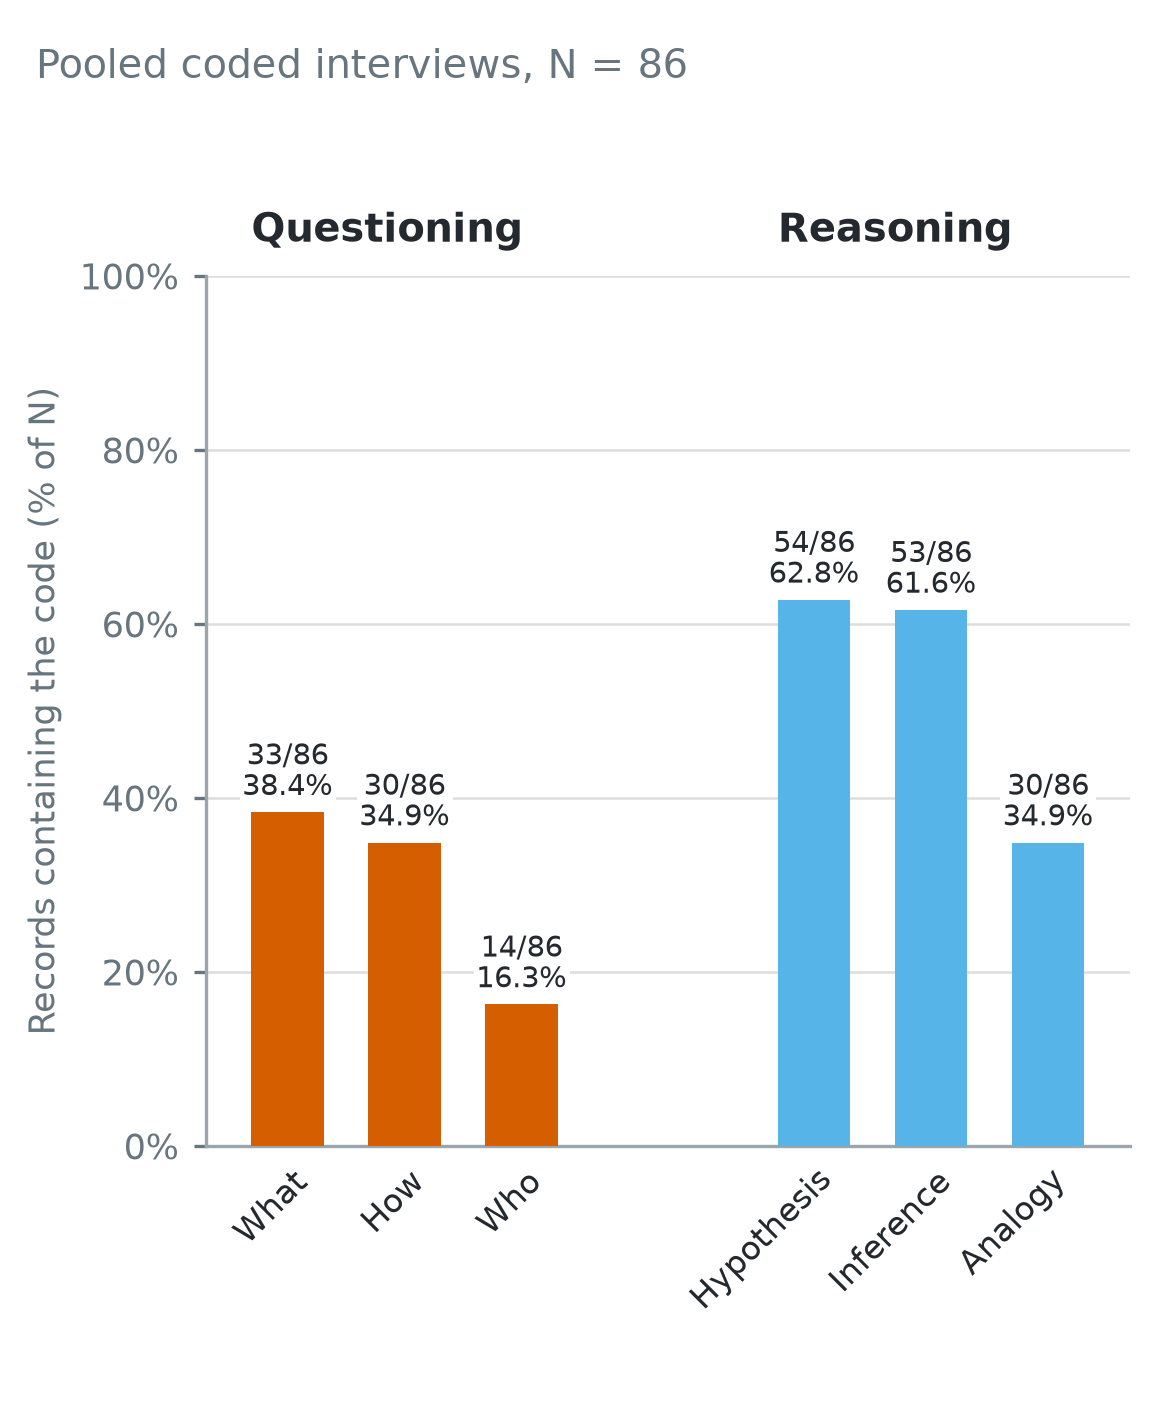
\includegraphics[width=\linewidth]{figures/fig_5_2_all_sites.png}
    \caption{Sensemaking strategies}
    \label{fig:strategies}
  \end{subfigure}
  \hfill
  \begin{subfigure}[t]{0.415\textwidth}
    \centering
    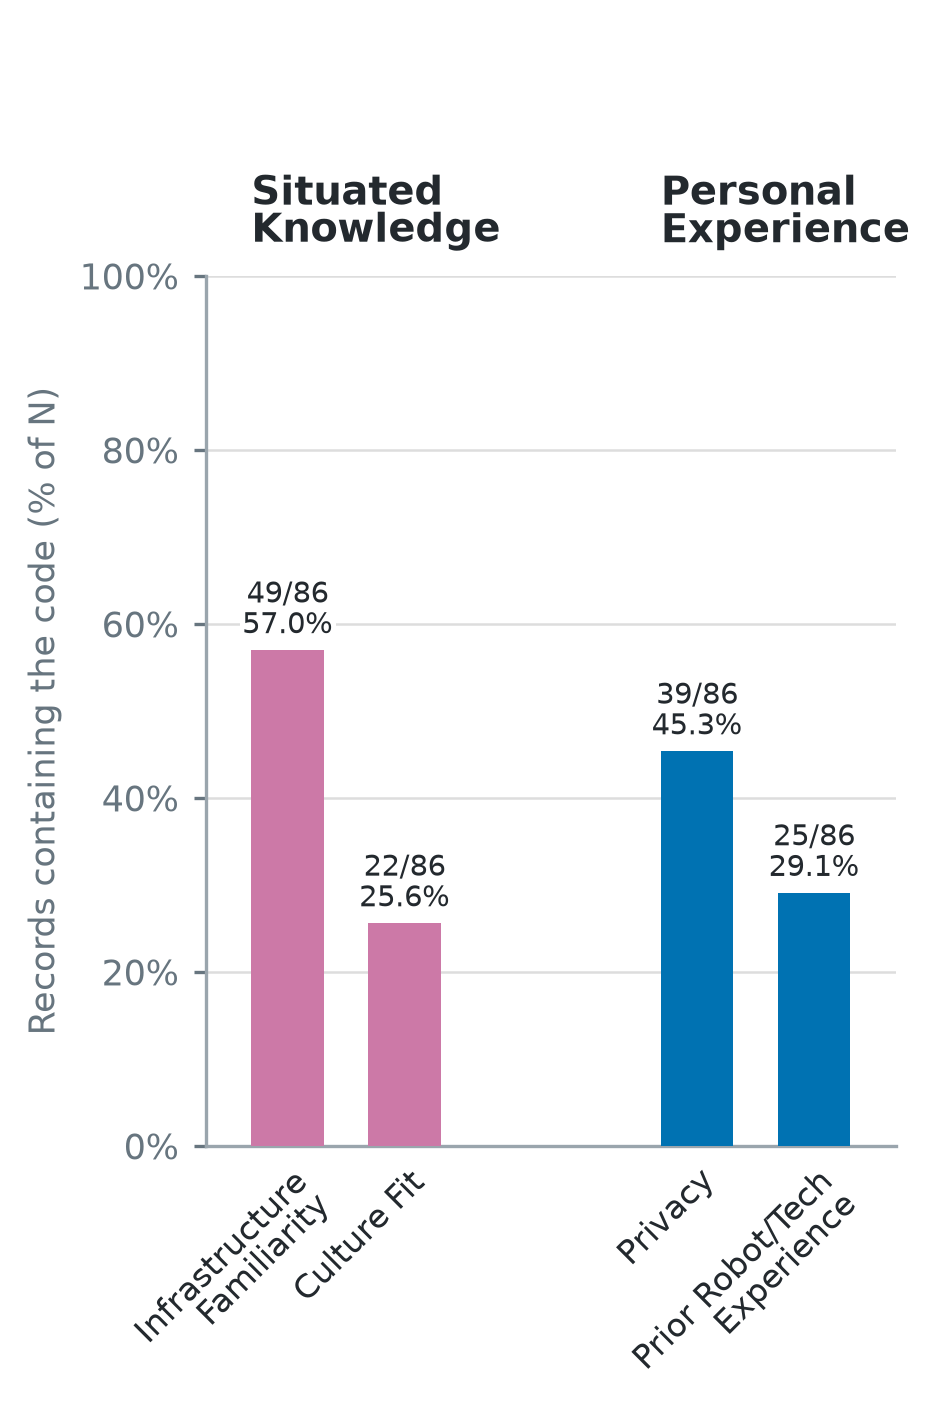
\includegraphics[width=\linewidth]{figures/fig_5_3_all_sites.png}
    \caption{Knowledge resources}
    \label{fig:resources}
  \end{subfigure}
  \caption{Prevalence of sensemaking codes across the pooled interview corpus ($N = 86$ interview records). (a)~Question-driven strategies (WHAT, HOW, WHO) and reasoning-based strategies (hypothesis, inference, analogy). (b)~Situated knowledge (infrastructure and familiarity, culture fit) and personal experience (privacy, prior robot or technology experience) that participants drew on. Bars show the share of records containing each code; codes are nonexclusive.}
  \Description{Two bar charts. Left chart, sensemaking strategies: What 38.4\%, How 34.9\%, Who 16.3\%; Hypothesis 62.8\%, Inference 61.6\%, Analogy 34.9\%. Right chart, knowledge resources: Infrastructure or familiarity 57.0\%, Culture fit 25.6\%; Privacy 45.3\%, Prior robot or technology experience 29.1\%.}
  \label{fig:sensemaking-all-sites}
\end{figure*}

To address \textbf{RQ3}, we examined the resources participants drew on when developing the interpretations described in Section~\ref{sec:process}. Similar forms of questioning and reasoning recurred across deployment sites, but the resources used to work through them varied. Some participants drew on knowledge of the setting itself, including existing infrastructure, familiarity with the community, and expectations about local behavior. Others relied on prior experience withrobots and related technologies and their expectation about the degree of privacy afforded by the site.  Among the resources identified in our analysis, we focus here on two broad families that were particularly relevant to the cross-site comparison: \emph{situated knowledge} and \emph{personal experience}. Situated knowledge was reflected through infrastructure or community familiarity and culture fit. Personal experience appeared through privacy and prior robot or technology experience. Figure~\ref{fig:sensemaking-all-sites}b visualizes the prevalence of the resource codes reported in this section.

\subsubsection{Situated Knowledge}
Situated knowledge concerned what participants knew about the deployment setting and how they used that knowledge to interpret the Trashbot. This included both the material and service conditions of the site and participants' understanding of its social and cultural context. Participants drew on existing infrastructure and services when judging whether the robot addressed a local need or duplicated what was already available. They also drew on familiarity with the community, including its history and expectations about how people at the site might respond to the robot.

\paragraph{Existing Infrastructure and Community Familiarity}
In 49 of 86 records (57.0\%), participants drew on infrastructure and community familiarity when interpreting the Trashbot. Participants frequently evaluated the Trashbot by comparing its proposed service with the sanitation resources already available around them. At Astoria Park, AP-09 welcomed the Trashbot because they think it is hard to find a nearby trash barrel: \emph{I do love the idea of them just roaming around...oftentimes you can't find a trash can.} LI-P03 made a similar judgment from the condition of existing infrastructure, noting that \emph{``a lot of the cans are overflowing or not available or not maintained correctly''} and therefore saw a technology intended to improve cleanliness as worthwhile. In these accounts, the Trashbot’s mobility made sense because it addressed a recognizable gap in the site’s existing sanitation services. Yet participants at the same site could read those services differently. LI-P22 saw little need for the Trashbot in Little Italy because \emph{``the community already have their cleaners and, you know, already have their porters that clean here every single day.''} Local infrastructure therefore shaped how participants judged the Trashbot’s usefulness, though not always in the same way. Participants also drew on their knowledge of this community history toward the interpretation of the Trashbot at the site. TP-P05 expressed that \emph{``it is not the ideal site''} by explaining that \emph{``you ain't in the safest park right now. This is [known as] drug city historically...you're going to get robbed by somebody around here''}. What counted as a suitable deployment site was thus anchored in participants’ understanding of the site as an existing social environment.

%might fit here instead: Similarly, LI-P17 \emph{there's a lot of, like, crackheads \ldots\ they like to knock stuff down \ldots\ Personally, over here, if it's more safer, it's more like being visualized, watched, here is perfect. Over there, it should be bad}.

\paragraph{Culture Fit}
In 22 of 86 records (25.6\%), participants used expectations about local norms, values, and behavior to judge whether the Trashbot fits that specific context. Whereas community familiarity concerned what participants knew about how a particular place functioned, culture fit concerned whether they saw the robot as compatible with how people there were expected to behave and with what the community appeared to value. AP-P04, for example, anticipated that \emph{``people don't respect [the robot]...you would probably have a much more effective deployment either in a wealthy community or [somewhere] outside of this region''}. Here, the concern was not simply knowledge of local conditions, but whether an unattended public robot would be treated in ways that allowed the service to work as intended. Culture fit could also be positive. CC-P11 saw the Trashbot as a visible sign that the site was \emph{``doing an active effort to keep it nice, the way I expect it to be,''} interpreting the robot as consistent with the environmental standards they associated with the place. LI-P21, by contrast, described the community they originally from as \emph{``very conscious about the environment''} and already relatively free of litter, making the Trashbot seem less necessary there. Their reference to the community culture assisted them to understand if the Trashbot was an appropriate addition to the site.

\subsubsection{Personal Experience}
Alongside with situated knowledge was anchored in the deployment setting, personal experience provided another source for interpreting the Trashbot. The two often worked together, as participants interpreted what they encountered through expectations and experiences formed elsewhere. These included prior experiences with cameras and surveillance, expectations about privacy, previous encounters with robots or related technologies, and familiar representations of robots. Because these experiences varied across individuals, participants at the same deployment site could interpret the same feature differently.

\paragraph{Privacy}
Participants (39/86, 45.3\%) used their understanding of privacy to judge the appropriateness of the Trashbot. Participants showed a variety of attitude towards the robot because of different attitude toward the privacy. For example, AP-P01 initially found the robot amusing but became more uneasy after noticing the camera, explaining \emph{``maybe it's a little invasive of privacy.''} CC-P16 shared a similar concern: \emph{``there is always the issue of privacy, right?...it's still not that nice to know that you are being constantly recorded''}. Other participants were less concerned about the privacy issue because they saw surveillance as already everywhere. CC-P06, for instance, said \emph{``I'm already pretty used to...phone tracking our activity across the apps, [and] being under surveillance all the time.''} Some participants also drew boundaries around where recording felt acceptable. CC-P05 distinguished public space from more private settings, saying they would object at \emph{``my workplace, or like my house, or my children's school''} but that \emph{``in the public place...I don't mind.''} These responses suggest that participants’ expectations about where and when surveillance was acceptable shaped whether the Trashbot’s camera, and by extension the robot itself, felt appropriate in the setting.

\paragraph{Prior Experience to Technology and Robots}
Participants also relyed on prior experience with robot to make sense of the Trashbot (25/86, 29.1\%). For some, this experience provided background knowledge for evaluating how the Trashbot should behave. LI-P33, who worked with robot in seminconductor manufacturing, focused on the robot's movement, suggesting that whether it would work depended on the \emph{``smoothness of the robot''} and noting that jerky motion could leave people unsure whether it was approaching them. Others compared the Trashbot with autonomous systems they already knew to anticipate possible interaction and problems. CC-P08 related to delivery robots, noting that \emph{``everyone wants to interact with it,''} while LI-P14 recalled encountering a robot dog in West Village,using that experience to interpret the Trashbot's novelty and the reactions it attracted from passersby. Participants also drew on familiar representations of robots in literature or science fiction movie to interpret the robot. For example, TP-P05 said the Trashbot \emph{``reminds me of the Jetsons. The Jetsons had a garbage can like [this],''} and AP-P04 described it as having \emph{``a mind of its own...[like] the T-1000...I do think that this is the future}. TP-P05 also invoked \emph{Judgment Day} and \emph{Skynet} when expressing distrust of technology. These prior encounters and references supplied expectations for how a robot might move, interact, or develop beyond what participants could observe from the Trashbot itself.
\section{Discussion}
\label{sec:discussion}

\subsection{The Interpretive Process of Public Robot Sensemaking}
\label{sec:service-justification}
% Sensemaking is a process, not an immediate evaluation
% Encountering makes the robot interpretively salient
% Interpreting is organized around WHAT, HOW, and WHO
    % Participants construct answers from available cues and reasoning strategies
% Situating turns an interpretation into a judgment about the robot’s place
% Imply and connect to local legibility

\begin{figure*}[t]
    \centering
    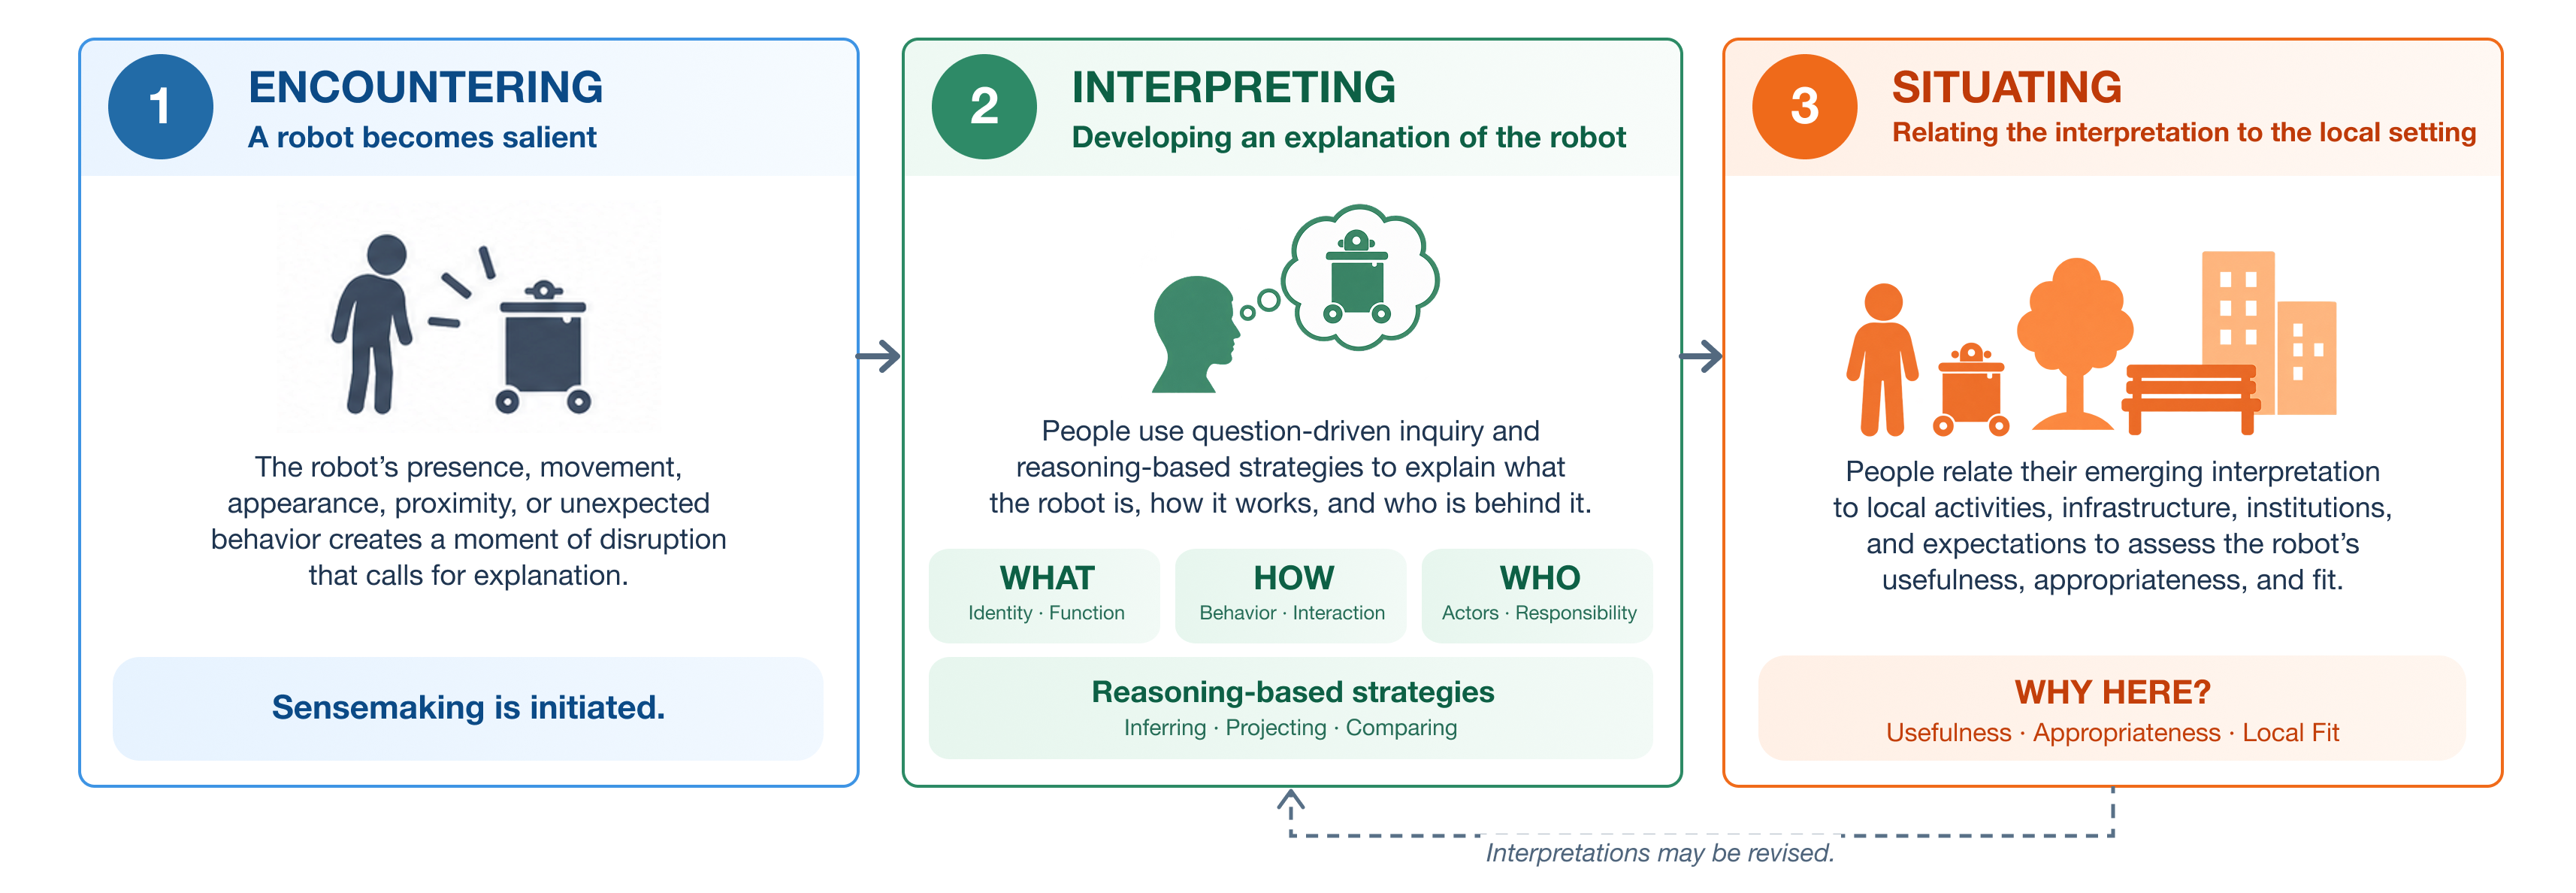
\includegraphics[width=0.95\textwidth]{figures/5.1.png}
    \caption{The interpretive process of public-robot sensemaking.}
    \Description{Conceptual diagram of the interpretive process of public-robot sensemaking, organized into three analytically related components arranged from left to right. The first stage, Encountering, shows a person noticing a robot and describes how the robot's presence, movement, appearance, proximity, or unexpected behavior can make it salient and initiate sensemaking. The second stage, Interpreting, shows people developing an explanation of the robot through question-driven inquiry and reasoning-based strategies. The questions are grouped as WHAT, concerning identity and function; HOW, concerning behavior and interaction; and WHO, concerning actors and responsibility. Reasoning strategies include inference, projection, and comparison. The third stage, Situating, shows people relating their emerging interpretation to local activities, infrastructure, institutions, and expectations in order to assess usefulness, appropriateness, and local fit. A dashed arrow from Situating back to Interpreting indicates that interpretations may be revised.}
    \label{fig:interpretive}
\end{figure*}

Our findings suggest that making sense of a public robot is not an immediate evaluation of whether the robot is useful or acceptable. Rather, it unfolds as an interpretive process through which people first notice the robot, work out what kind of system they are encountering, and then consider what that system means in relation to the place around them. As illustrated in Figure~\ref{fig:interpretive}, we characterize this process as three analytically distinct moments: \emph{encountering}, \emph{interpreting}, and \emph{situating}, a structure that emerged from our analysis and that accordingly organizes how we report the findings. Encountering makes the robot salient as something that calls for explanation; interpreting involves questioning and reasoning through the robot’s identity, operation, and social organization, with recurring concerns around WHAT, HOW, and WHO; and situating relates these emerging interpretation into relation with the local setting, seeking to answer WHY HERE?

This account is consistent with sensemaking as the interpretive work through
which people render an unfamiliar situation intelligible
~\cite{weick2005organizing}.  The Trashbot's familiar trash-can form provided an initial cue, but its movement, camera, proximity, and apparent autonomy made that cue insufficient to explain the system as a whole. This ambiguity exposes interpretive work that is often implicit in public HRI. Prior research has examined different parts of this problem: legibility concerns how observers infer a robot's goals from its behavior~\cite{dragan2013legibility}; mental-model research examines how people form expectations about autonomous systems from incomplete evidence~\cite{paepcke2010judging,riek2012wizard}; field studies show pedestrians working out how to approach, avoid, assist, or coordinate with unfamiliar robots~\cite{pelikan2024encountering,dobrosovestnova2022little,weinberg2023sharing}; and privacy research raises questions about who is sensing, who receives the resulting data, and for what purpose~\cite{denning2014insitu,dietrich2026bystander}.

Seen together, these concerns align with the recurring WHAT, HOW, and WHO questions in our data. WHAT concerns the robot's identity and purpose, extending legibility beyond inferring an immediate motion goal; HOW concerns how its behavior, sensing, and interaction are produced; and WHO locates the robot within a broader socio-technical arrangement of operators, institutions, data recipients, and responsible stakeholders. These questions are especially consequential for bystanders, who encounter robots without prior instruction or an assigned relationship to them~\cite{scholtz2003theory,rosenthal2020forgotten}. Because definitive answers were rarely available, participants worked provisionally: they inferred from visible and behavioral cues, projected possible actions and consequences, and compared the Trashbot with familiar technologies and situations. This resembles the inferential work described in legibility and mental-model research~\cite{dragan2013legibility,paepcke2010judging}, while also drawing on prior experience and shared knowledge~\cite{clark1996using,weick2005organizing}. Questioning and reasoning are therefore complementary: questions identify gaps in an emerging account, while inference, projection, and comparison provide ways of filling them.

Yet resolving WHAT, HOW, and WHO did not settle the encounter. Participants also related these provisional interpretations to the activities, infrastructure, institutions of the surrounding place, echoing prior work showing how robots become embedded within existing workflows, social arrangements, and physical environments ~\cite{mutlu2008robots}. We characterize this as \emph{situating}. WHY HERE? is therefore not simply a fourth question equivalent to WHAT, HOW, and WHO: it asks whether a system understood in those terms makes sense in this particular setting. This move is consistent with situated accounts in which meaning is produced in relation to the circumstances of action~\cite{suchman1987plans}, and with work arguing that public robots must be understood within the particular social organization of the places they enter~\cite{pelikan2025localism,bu2025making}. Public-robot sensemaking thus moves from making the robot intelligible to making its presence locally intelligible, providing the basis for the concept of \emph{local legibility} that we discuss next.

\subsection{Local Legibility as a Basis for Public Robot Interpretation}
\label{sec:local-legibility}

% The findings suggest an extension of legibility as a design concern. 
In HRI, legibility has often referred to whether an observer can infer a robot's immediate goal from its behavior or motion~\cite{dragan2013legibility}. Our findings suggest that, for public service robots, legibility is a basis for the broader interpretive process we discussed in Section~\ref{sec:service-justification}. Participants were not only trying to make sense what the Trashbot was about to do in the moment; they frequently used questioning and reasoning to interpret its broader presence, then situated these interpretation within the local setting. We therefore call a public service robot \emph{locally legible} when people can understand its role within the place where they encounter it. This includes its immediate function and interaction cues, along with the institution responsible for it, the service it provides, the meaning of its sensing or recording, and its relation to existing infrastructure and labor. This extends legibility from a relation between behavior and interpreted goal to a relation among the robot, its broader service arrangement, and the site in which it exists~\cite{while2021urban}.

\paragraph{Accountable attribution} For a public robot to be locally legible, people should be able to identify the stakeholders responsible for its presence and operation. This corresponds to the WHO questions in our findings, through which participants sought to locate the Trashbot within a broader social arrangement. Prior work on privacy-sensitive robotics and bystander privacy has emphasized that public robots affect people who may never choose to interact with them, making questions of who collects, receives, and governs sensed information~\cite{rueben2018themes, dietrich2026bystander}. Dietrich et al., in particular, show how robotic agency can complicate the attribution of actor roles within information flows. In our study, the Campus Café research setting offered participants a plausible institutional attribution, leading them to interpret the Trashbot as a student or research project associated with the surrounding institute. At street and park sites, participants drew on familiar service arrangements, including city sanitation and park management, to infer its affiliation. The responsible institution may need to be identifiable to people who directly interact with the robot, as well as to bystanders who encounter it without choosing to engage. Earlier organizational HRI studies similarly show that robotic services become embedded in existing workflows and relationships beyond the immediate user interaction~\cite{mutlu2008robots,lee2012ripple}. The robot's service role also has to make sense alongside workers and infrastructure already performing related functions. Institutional attribution is therefore part of the public interface: deployments should make clear who is responsible for the robot and how that responsibility relates to the existing division of work and service already in place.

\paragraph{A recognizable local need} 
Local legibility also requires that people can understand \textit{why} the robot belongs in the place where they encounter it and what problem its service helps address. Before people can judge whether a robot is needed \emph{here}, they first need to understand what service it provides and how that service works. In our deployments, confusion was therefore understandable and expected because the Trashbot did not always make its function or intended interaction apparent on its own. Our participants then drew on situated knowledge of the surrounding infrastructure, activities, and local norms to judge whether that service made sense in the site. The same mobile trash service could appear useful where receptacles were distant or poorly maintained, yet unnecessary where fixed bins and cleaners already provided adequate sanitation in the space. Participants also drew on their familiarity with local norms and expected reactions of others to judge whether the Trashbot would be accepted, respected, and used as intended, and thus whether its service could realistically work in that site. This aligns with prior work on localism in public robot design, which argues that public space is not a uniform setting but is organized through site-specific activities, norms, and social relations~\cite{pelikan2025localism}. Related field studies likewise show how cultural knowledge, communal common ground, and everyday activity shape the interpretation of robots in public settings~\cite{bu2025making}. Our findings extend this work by showing how people use such situated knowledge to assess both the need for a robot's service and whether that service can plausibly become part of the setting. A robot's presence may therefore become easier to make sense of when its features and behavior, together with cues from the surrounding environment, point to a recognizable local problem and a role that people can see working there.

\paragraph{Accommodating individual differences} 
Local legibility is also shaped by differences among the people who share a place and should not imply that a place has one single shared interpretation of a public robot. Even within the same site, our participants drew on different prior experiences, associations, and expectations when making sense of the Trashbot. Associations with benevolent or threatening fictional robots, for example, contributed to contrasting interpretations, while recording practices that seemed acceptable to some participants and raised concerns for others. Prior work has documented the cultural and experiential resources people draw on when interpreting public robots~\cite{bu2025making}, as well as variation in how bystanders respond to recording technologies in public settings~\cite{denning2014insitu}. Our findings bring these perspectives into account of local legibility by showing that shared exposure to the same local infrastructure, practices, and robot does not guarantee a shared interpretation. Adapting a robot to a site's infrastructure and practices may still leave individual concerns unresolved. Therefore, local legibility should be treated as an ongoing process of explanation and adjustment. Alongside making the robot's purpose and recording practices explicit, deployments could offer ways to request further information, decline interaction, and communicate concerns that inform changes to robot behavior or operating practices. These mechanisms would help deployments respond to the different people who share a place.

\subsection{Design Implications for Locally Legible Deployment} 
\label{sec:deployment-relationship} 
Building on the three factors underlying local legibility discussed in Section~\ref{sec:local-legibility}, we propose three corresponding design implications: make the institution identifiable, engage with the community, and disclose sensing and data practices. We address these implications in the same order, translating each factor into actionable guidance for designing and operating public robots.

\paragraph{Make the institution identifiable} Prior work has recommended signage and messaging that explain who owns and services public robots~\cite{bu2025making}. Our findings suggest that the design of this information should account for the institutional cues already available at each deployment site. To support accountable attribution as a dimension of local legibility, we recommend placing clearly visible institutional identification on the robot or nearby that is explicitly associated with it. At sites with a recognizable institutional affiliation, such as a university campus, a familiar logo accompanied by a brief statement of the institution's role may help confirm people's understanding of who is responsible for the robot. At sites where this affiliation is less apparent, signage should provide more explicit information about the organization operating the robot, its responsibilities, and whom people can contact with questions or concerns. Visible staff could supplement this information by explaining the deployment and clarifying responsibility. Deployment teams should assess whether these cues allow people unfamiliar with the project to identify the responsible institution.

\paragraph{Engage with the community} 
Community engagement should help establish a locally recognizable role for the robot. Our findings show that participants evaluated the Trashbot through their knowledge of existing services and everyday activities. In Little Italy, participants' familiarity with daily cleaning raised questions about the Trashbot's need and additional value to the community, while participants at Astoria Park identified the Trashbot potential uses to fix the site's lack of trash barrels issue. These accounts suggest that local legibility depends partly on whether the robot's placement and operation communicate a purpose that makes sense locally. Building on prior work on co-designing public robots and situated community engagement~\cite{han2024codesign,yavoayalon2023cxr}, we suggest combining site walkthroughs with discussions of proposed deployment scenarios. Residents, workers, site managers, and regular users could identify existing service arrangements, periods of unmet need, and activities that robot operation might disrupt. Using maps, demonstrations, or enactments, deployment teams could then invite participants to interpret specific encounters: what would a robot approaching this location appear to be doing, why would its presence make sense here, and how would it affect the people already using or maintaining the space? These discussions should inform concrete decisions about routes, operating hours, approach behavior, and the division of work between the robot and existing service providers. 

\paragraph{Make sensing and data practices visible} 
Local legibility requires more than disclosing of what a robot is sensing or recording. People should also be able to understand what is collected, why it is collected, who can access it, and how concerns about those practices can be raised. Prior work has highlighted bystander privacy challenges and the need to accommodate changing privacy preferences~\cite{rueben2018themes, dietrich2026bystander}. To support local legibility, we recommend pairing visible explanations of sensing practices with a clearly advertised channel for questions and feedback throughout a deployment. This channel could include contact information on the robot or nearby signage, a feedback form, and opportunities to speak with deployment team. It should support both individual and community-level concerns.  At the individual level, people should be able to request clarification, raise concerns about a particular encounter, or communicate that they do not wish to be recorded. The team should explain how these requests will be handled and communicate any resulting changes. At the community level, recurring concerns could inform changes to sensing coverage, recording schedules, or data access. Maintaining this exchange would allow both privacy practices and their explanations to remain responsive to the people who encounter the robot.
\section{Limitations and Future Work}
\label{sec:limitations}

\paragraph{Contextual transferability.}
The five deployments span different public and quasi-public settings, but they all took place in New York City and involved the same sanitation-oriented service concept. The specific institutions, infrastructure, and local expectations that participants drew on are therefore tied to this municipal and service context. Future work should examine whether the recurring sensemaking questions identified here also appear in other cities, cultural settings, and public-service domains, and how the resources used to answer those questions change across contexts. Our interview corpus also provides uneven coverage of multilingual encounters because some non-English speech was not transcribed reliably. This limits the accounts represented in our analysis and points to the need for stronger multilingual support in future field studies.

\paragraph{Place-level and participant-level variation.}
Our analysis foregrounds the knowledge participants drew from the deployment setting, but participants also brought their own experiences to the encounter. Occupation, familiarity with the site, prior experience with robots and other technologies, and experience in other neighborhoods or institutions could all inform how a participant interpreted the Trashbot. The present study does not systematically separate these participant-level resources from knowledge associated with the site. Future work could examine how personal experience and place-based knowledge combine when people interpret public robots, including cases in which they point toward different conclusions.

\paragraph{Wizard-of-Oz and autonomous deployment.}
The Trashbots were remotely operated throughout the deployments, while participants initially encountered each robot as apparently autonomous. This operating arrangement allowed us to use the same platform design and operating protocol across sites, but the study captures sensemaking around perceived autonomy rather than sustained interaction with fully autonomous systems. Autonomous operation may introduce navigation failures, delays, recovery behavior, and other cues that affect how people read the robot's actions and judge its competence or appropriate role. Longer deployments may also change these interpretations as people become familiar with the robot and its institutional context. Future work should examine whether the sensemaking strategies and factors identified here persist under autonomous and longer-term deployment.
\section{Conclusion}
\label{sec:conclusion}

We studied how people read Trashbots across five deployment sites spanning, one in each New York City borough. Our findings show that people did not understand a public robot from its form or behavior alone. They worked out what the robot was doing by using question-driven and reasoning-based strategies to make sense of their presence. These strategies included recurring WHAT, HOW, and WHO questions as well as inference, projection, and comparison. How participants read the robots' actions was often shaped by situated knowledge of the encounter site and by personal experience brought to the interaction.

These findings motivate \emph{local legibility} as a design objective for public HRI. We identified how local legibility emerges through the interpretive process by showing how people combine cues from the robot with site-specific knowledge and personal experience to make sense of its presence. We proposed design implications for making public robot deployments more locally legible, including disclosing the responsible institution and sensing practices, relating the robot's service to existing infrastructure and activities, and accounting for the expectations that people within the community bring to the encounter. Because the same robot can be read differently across and within deployment sites, designing for local legibility also requires making the service arrangement understandable in place while recognizing that no single site-level explanation will resolve individual's interpretation.

Longer-term and fully autonomous deployments are still needed to examine how local legibility develops over time as people become familiar with a robot, experience its failures and adaptations, and form expectations for it. We hope our work can help extend discussions of legibility in public HRI beyond making a robot's individual actions understandable toward considering how its broader service role, responsibility, practices, and fit with the surrounding place become intelligible to the people who share the spaces in which it is situated.




\bibliographystyle{ACM-Reference-Format}
% Separate reference entries for easier scanning in the review manuscript.
\setlength{\bibsep}{4pt plus 1pt minus 1pt}
\bibliography{reference}

%% Appendix: goes after the bibliography (acmart convention).
\appendix

\section{Deployment Sites}
\label{app:sites}

% Recommendation: rewrite Sites as setting description and restate the
% load-bearing facts about each place in our own voice: what it looks like,
% who is there, who maintains it, its reputation, how we got access, and
% where the team stood.
\textbf{Tappen Park (Staten Island)} is a neighborhood park in Stapleton near a commercial district and the waterfront. Visitors use the park largely for sitting, talking, and spending time rather than organized recreation. Fixed trash receptacles are located around the park but are not distributed continuously through the open seating areas. The surrounding area also carries a documented reputation for public-safety concerns, including drug activity~\cite{sifentanyltaskforce2024}. We deployed TrashBot around the open lawn and paved paths, with the operator seated on a nearby bench.

\textbf{Astoria Park (Queens)} is a large riverside leisure park on the East River used for running, cycling, family outings, sunbathing, and other outdoor recreation. We deployed TrashBot near the swimming-pool entrance, along the riverside walk, and beside the skatepark. These areas placed the robot among parents with children, cyclists, and people sitting or lying on lawns and benches. Fixed trash receptacles were distributed across the park but often required walking some distance from the recreation areas. The site was covered by the same Parks Department permit, and the operator worked from a bench at the edge of the deployment area.

\textbf{Little Italy (Bronx)} is a dense commercial corridor centered on Arthur Avenue in Belmont and historically associated with the borough's Italian immigrant community~\cite{apa2016arthuravenue, helmreich2023bronx}. Restaurants, shops, market activity, and heavy pedestrian traffic occupy the corridor, and sanitation is visibly organized through local cleaning crews, porters, and fixed street receptacles. We deployed TrashBot in the plaza outside a pizzeria on the corridor. Access was arranged through the executive director of the neighborhood business association, who introduced the research team to nearby business owners.

\textbf{Campus Café (Manhattan)}The Manhattan deployment took place at a café beside a research institute. The café and its outdoor seating area are used by institute affiliates, local residents, and visitors. Deployment permission were granted by the institute's campus safety department.

\textbf{Brooklyn Navy Yard (Brooklyn)} is an access-controlled industrial and commercial campus used primarily by people working at organizations based there. Access was arranged
through a member of a community engagement group, who initially invited the research team to a community event. Permission to deploy TrashBot at the site was subsequently granted.




\end{document}
